\documentclass[12pt,a4paper,openany,oneside]{report}
\usepackage[utf8]{vietnam}
\usepackage{amsmath, amsthm, amssymb,amsxtra,latexsym,amscd,graphpap,makeidx}
\usepackage{pgf,tikz}
\usepackage{mathrsfs}
\usetikzlibrary{arrows}
\usepackage{float}
\usepackage{algorithm}
\usepackage{algpseudocode}
\usepackage{graphicx}
\usepackage{array,tabularx,longtable,multicol,indentfirst,fancyhdr}
\usepackage[mathscr]{eucal}
\usepackage[top=3.5cm, bottom=3.0cm, left=3.5cm, right=2cm]{geometry}
\usepackage{fancybox}
\usepackage{listings}
\usepackage{xcolor}
\usepackage[utf8]{inputenc}
\usepackage{hyperref}
\usepackage[strings]{underscore}



\renewcommand{\chaptername}{Chương}
\renewcommand\bibname{Tài liệu tham khảo}

\pagestyle{fancy}
\fancyhf{}
\fancyhead[L]{\nouppercase{\leftmark}} 
\fancyhead[R]{\thepage} 
\fancyfoot[C]{} 
\renewcommand{\headrulewidth}{0.4pt}
\renewcommand{\footrulewidth}{0pt} 

\begin{document}

\newgeometry{top=2.0cm,bottom=3.0cm,left=3.0cm,right=2.8cm}
\setlength{\fboxrule}{1.5pt}
\thisfancypage{\setlength{\fboxsep}{10pt}\setlength{\shadowsize}{0pt}\doublebox}{}

\begin{titlepage}
\fontsize{14pt}{14pt}\selectfont \baselineskip 0.65cm
\thispagestyle{empty}
\begin{center}
{HỌC VIỆN CÔNG NGHỆ BƯU CHÍNH VIỄN THÔNG}\\
\textbf{\MakeUppercase{KHOA CÔNG NGHỆ THÔNG TIN I}}\\
\centerline{--------------------o0o--------------------}  
\end{center}

\begin{figure}[H]
	\begin{center}
		
\includegraphics[width=6cm]{logo.png}
	\end{center}
\end{figure} 
 
\vspace{0.5cm}
\begin{center}
\textbf{\MakeUppercase{\LARGE \bf BÁO CÁO BÀI TẬP LỚN}}\\ 
\end{center} 



\vspace{0.1cm}
\begin{center}
	\textbf{Môn: Kiến trúc máy tính}\\[0.5cm]
	\textbf{Chủ đề: Lập trình hợp ngữ Assembly và phân tích }\\[0.01cm]
    \textbf{hệ thống bộ nhớ}\\[0.5cm]
	\textbf{Giảng viên: Trần Tiến Công}
\end{center}

\vspace{1cm}
\hspace{3cm}
\begin{tabular}{ll}
    Nguyễn Trường Thái & B23DCCN747 \\
	Hà Duy Khánh & B23DCCN426 \\
	Vũ Quang Huy & B23DCCN412 \\
	Lê Huy Hải & B23DCCN272 \\
\end{tabular}

\vfill
\begin{center}
{{\bf Hà Nội, 5/2025}}
\end{center}
\end{titlepage}


\restoregeometry
\pagestyle{fancy}
\pagenumbering{roman}
\fontsize{13pt}{13pt}\selectfont \baselineskip 0.75cm 

\newpage
\thispagestyle{empty}
\tableofcontents


\newpage 
\addcontentsline{toc}{chapter}{\bf  Danh sách hình vẽ} 

\listoffigures


\newpage
\thispagestyle{plain}
\begin{center}
	{\LARGE
		{\bf Danh sách các ký hiệu và chữ viết tắt}}
\end{center}
\addcontentsline{toc}{chapter}{Danh sách các ký hiệu và chữ viết tắt}
\vspace{1.25cm}
{\fontsize{13}{13}\selectfont
	\begin{tabular}{ll}
		CPU & Central Processing Unit (Đơn vị xử lý trung tâm)\\
		RAM & Random Access Memory (Bộ nhớ truy cập ngẫu nhiên)\\
		ROM & Read-Only Memory (Bộ nhớ chỉ đọc)\\
		IP & Instruction Pointer (Con trỏ lệnh)\\
		DS & Data Segment (Đoạn dữ liệu)\\
		SS & Stack Segment (Đoạn ngăn xếp)\\
		CS & Code Segment (Đoạn mã)\\
		BP & Base Pointer (Con trỏ cơ sở)\\
		SP & Stack Pointer (Con trỏ ngăn xếp)\\
		SI & Source Index (Chỉ mục nguồn)\\
		HĐH & Hệ điều hành\\
	\end{tabular}
}

\newpage
\pagenumbering{arabic} 
\pagestyle{fancy} 

\chapter*{Mở đầu}
\addcontentsline{toc}{chapter}{\vspace*{-8pt}  Mở đầu} 

Trong lĩnh vực khoa học máy tính, lập trình hợp ngữ Assembly là một trong những kỹ năng nền tảng quan trọng, giúp người học hiểu sâu về cách thức hoạt động của máy tính ở mức thấp. Ngôn ngữ Assembly là ngôn ngữ lập trình cấp thấp, gần với mã máy nhưng vẫn có thể đọc hiểu được đối với con người. Việc nắm vững Assembly giúp lập trình viên hiểu rõ hơn về kiến trúc máy tính, quản lý bộ nhớ, và tối ưu hóa hiệu suất chương trình.

Báo cáo này tập trung vào hai phần chính: phần thứ nhất trình bày các bài tập lập trình hợp ngữ Assembly, và phần thứ hai phân tích khảo sát hệ thống bộ nhớ. Trong phần lập trình Assembly, chúng tôi thực hiện nhiều bài tập đa dạng như chuyển đổi ký tự thường thành hoa, chuyển đổi giữa các hệ cơ số, tính toán số học, và xử lý chuỗi. Mỗi bài tập đều được minh họa bằng mã nguồn và kết quả thực thi, giúp người đọc hiểu rõ cách thức hoạt động của từng chương trình.

Phần phân tích khảo sát hệ thống bộ nhớ tập trung vào việc tìm hiểu cấu hình máy tính và cơ chế quản lý bộ nhớ. Chúng tôi sử dụng các công cụ như CPU-Z để khảo sát thông số kỹ thuật của CPU, cache, RAM, và các thiết bị lưu trữ. Đồng thời, chúng tôi cũng sử dụng công cụ debug để theo dõi và phân tích nội dung các thanh ghi như IP, DS, ES, SS, CS, BP, SP, từ đó hiểu rõ hơn về cơ chế quản lý bộ nhớ của hệ thống.

Mục tiêu của báo cáo này là giúp người đọc hiểu sâu hơn về lập trình Assembly và kiến trúc máy tính, đồng thời cung cấp các ví dụ thực tế về cách thức áp dụng kiến thức này vào việc phát triển và tối ưu hóa phần mềm. Chúng tôi hy vọng rằng báo cáo này sẽ là tài liệu tham khảo hữu ích cho sinh viên và những người quan tâm đến lĩnh vực lập trình cấp thấp và kiến trúc máy tính.

\chapter{Lập trình hợp ngữ Assembly}

\section{Bài tập của Nguyễn Trường Thái}

\subsection{Chuyển ký tự thường thành ký tự hoa}
Chương trình hợp ngữ Assembly cho phép nhập 1 ký tự viết thường và in ra màn hình chữ hoa của ký tự đó.

\begin{figure}[H]
    \centering
     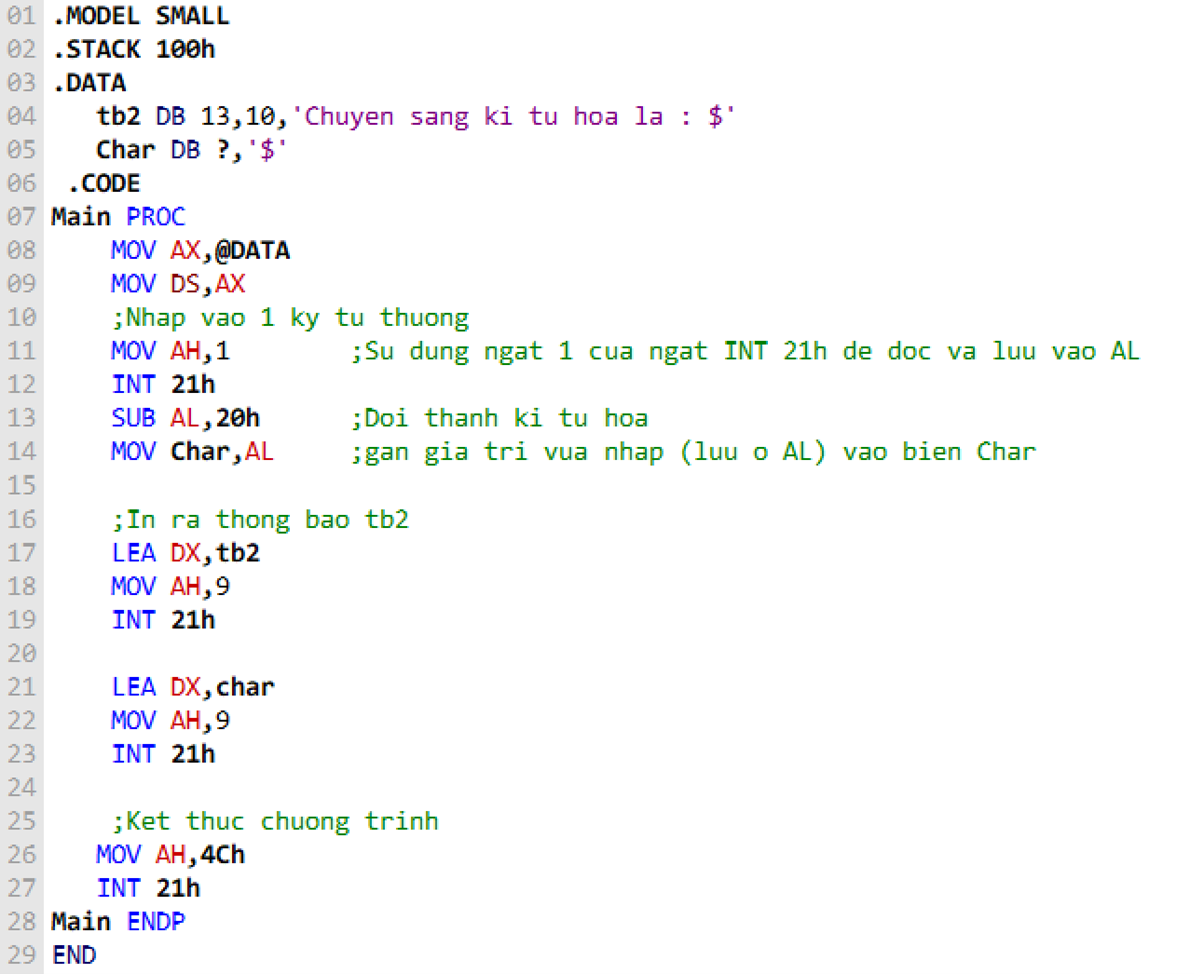
\includegraphics[width=0.9\textwidth]{Thái/Picture1.png}
    \caption{Mã nguồn in ra ký tự theo dạng viết hoa}
\end{figure}


\begin{figure}[H]
    \centering
     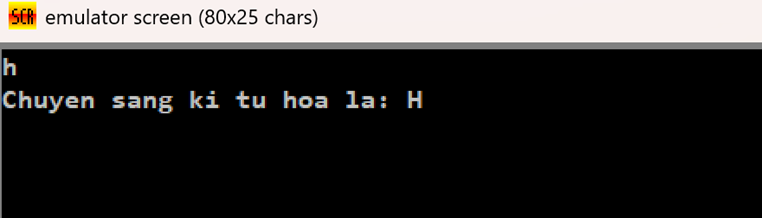
\includegraphics[width=0.8\textwidth]{Thái/Picture2.png}
    \caption{Giao diện in ra ký tự theo dạng viết hoa}
\end{figure}

\subsection{Chuyển số từ hệ cơ số 10 sang hệ cơ số 16}
Chương trình hợp ngữ Assembly chuyển một số từ hệ cơ số 10 sang hệ cơ số 16 (Hexa).

\begin{figure}[H]
    \centering
    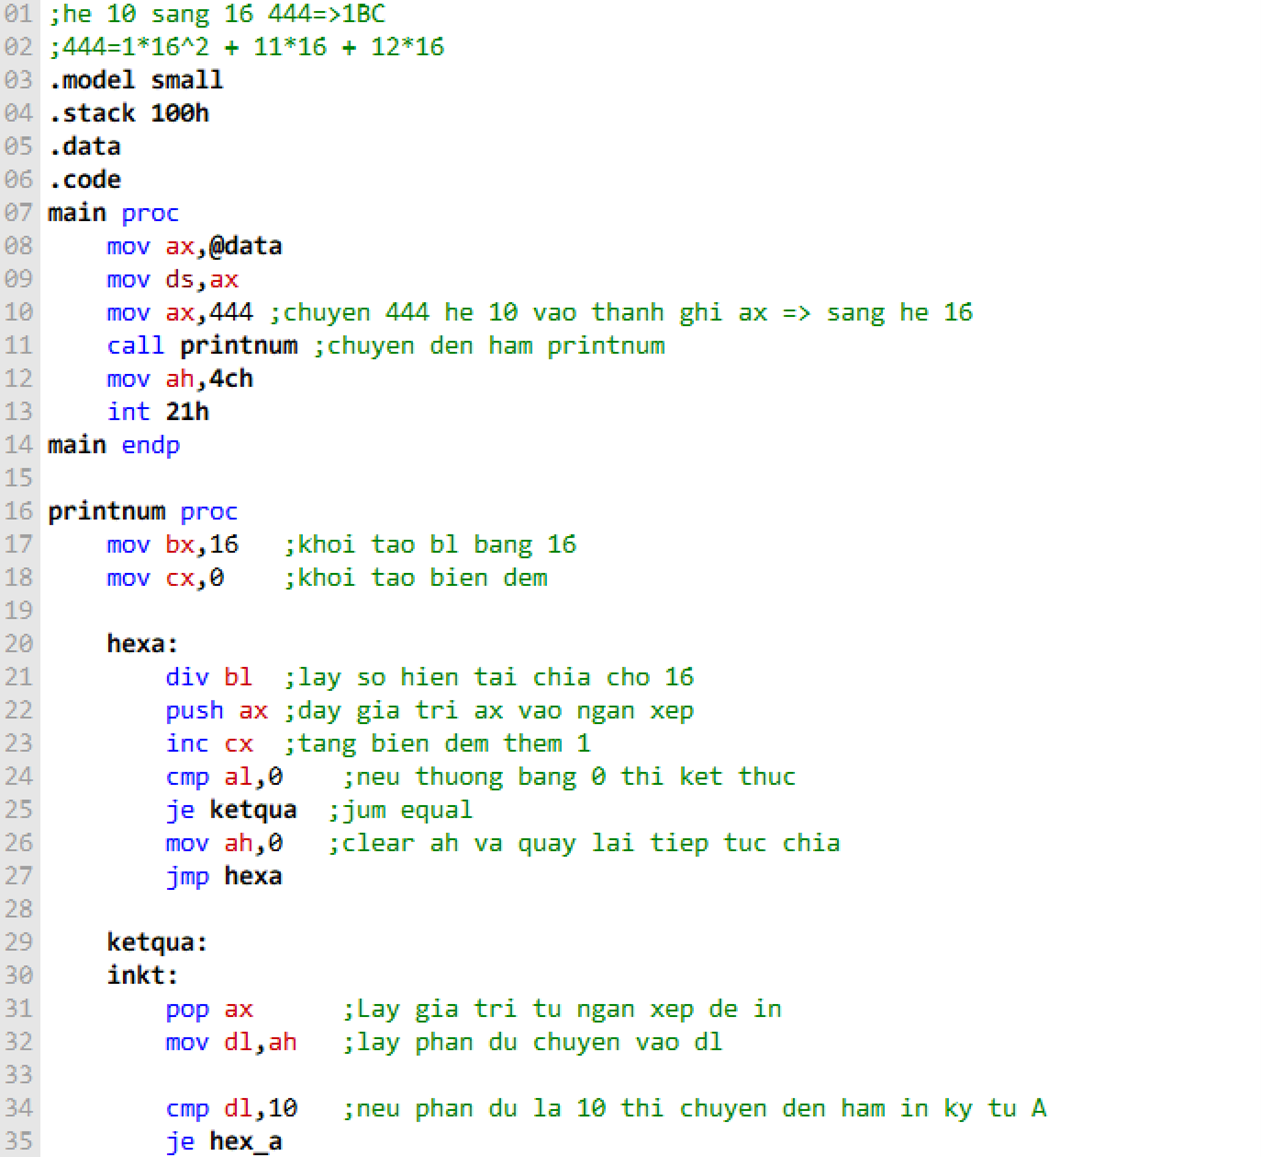
\includegraphics[width=0.9\textwidth]{Thái/Picture3.png}
\end{figure}

\begin{figure}[H]
    \centering
    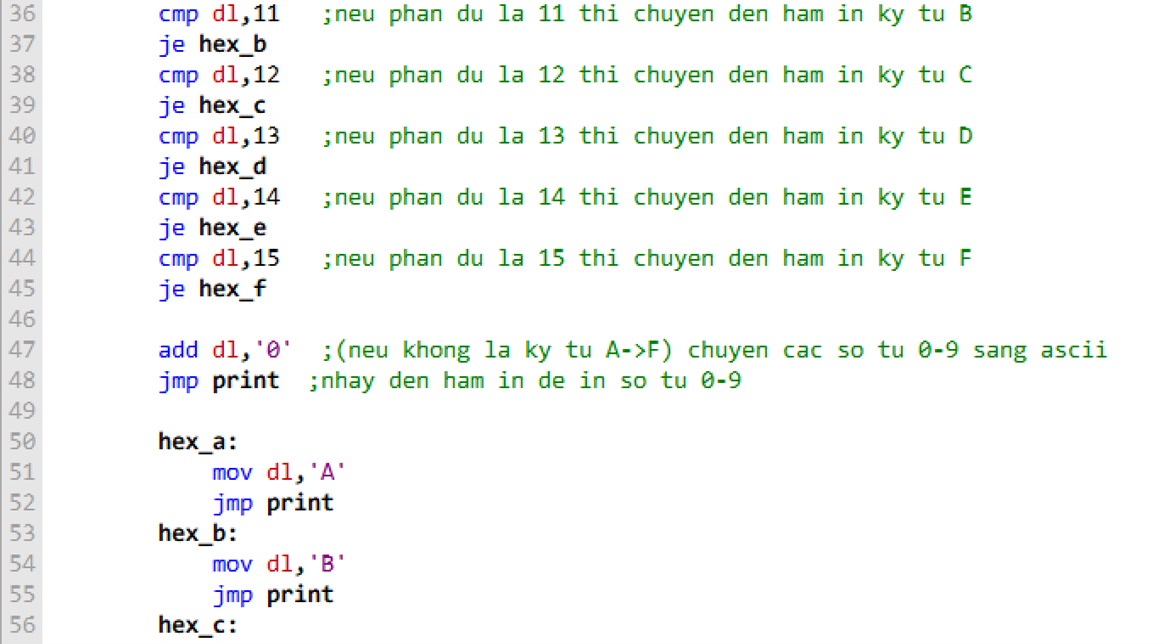
\includegraphics[width=0.9\textwidth]{Thái/Picture4.png}
     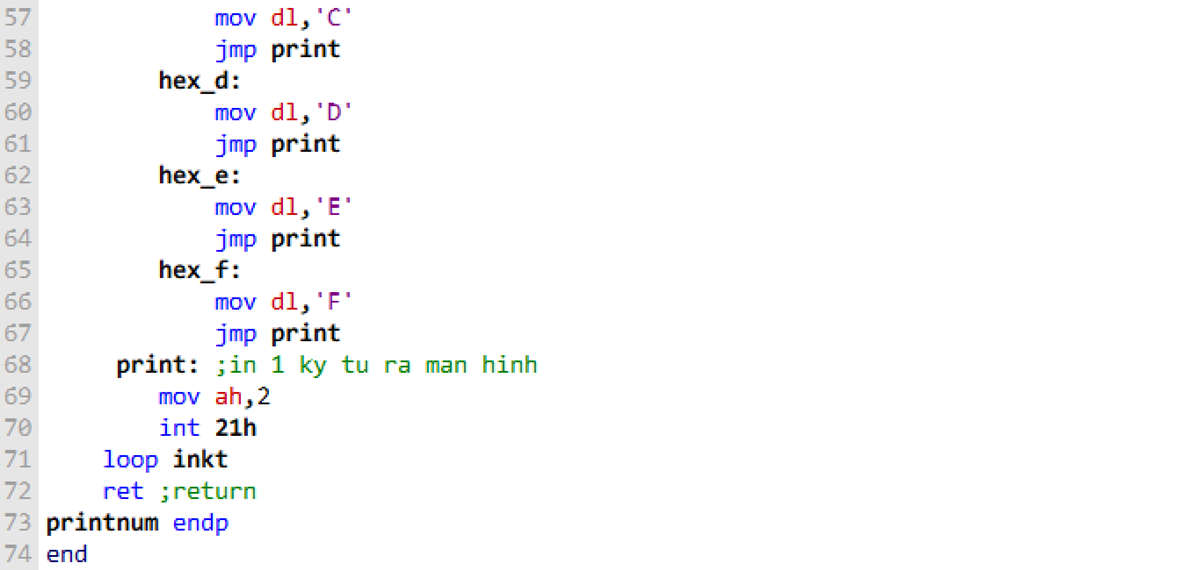
\includegraphics[width=0.9\textwidth]{Thái/Picture5.png}
    \caption{Mã nguồn in ra chuyển số 444 từ hệ cơ số 10 sang hệ cơ số 16}
\end{figure}


\begin{figure}[H]
    \centering
      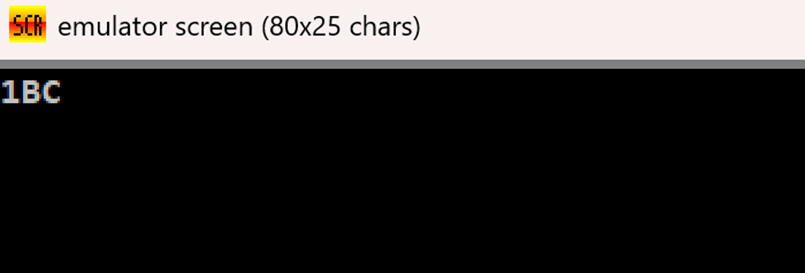
\includegraphics[width=0.9\textwidth]{Thái/Picture6.png}
    \caption{Giao diện in ra giá trị 444 từ hệ cơ số 10 sang hệ cơ số 16}
\end{figure}

\subsection{Tính tổng 2 số kiểu word}
Chương trình hợp ngữ Assembly tính tổng 2 số kiểu word.

\begin{figure}[H]
    \centering
    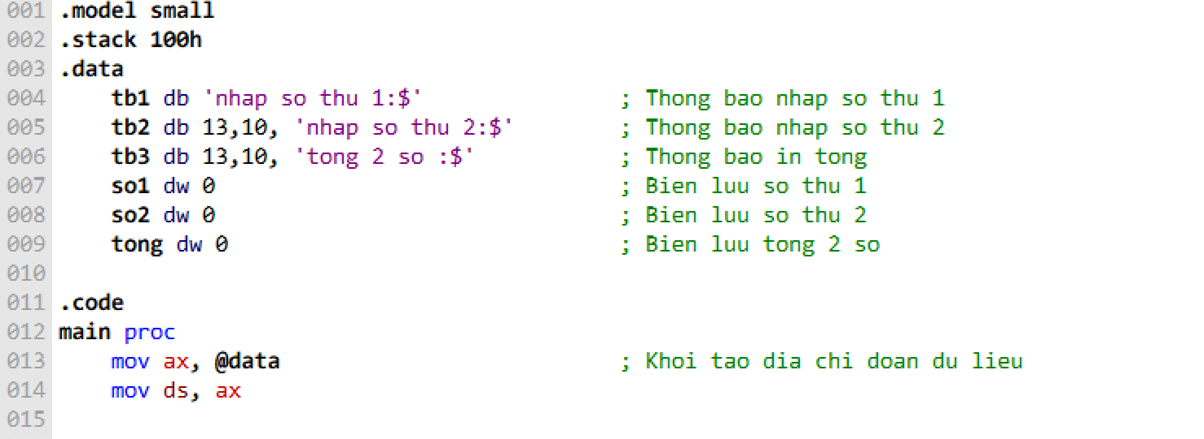
\includegraphics[width=0.9\textwidth]{Thái/Picture7.png}
      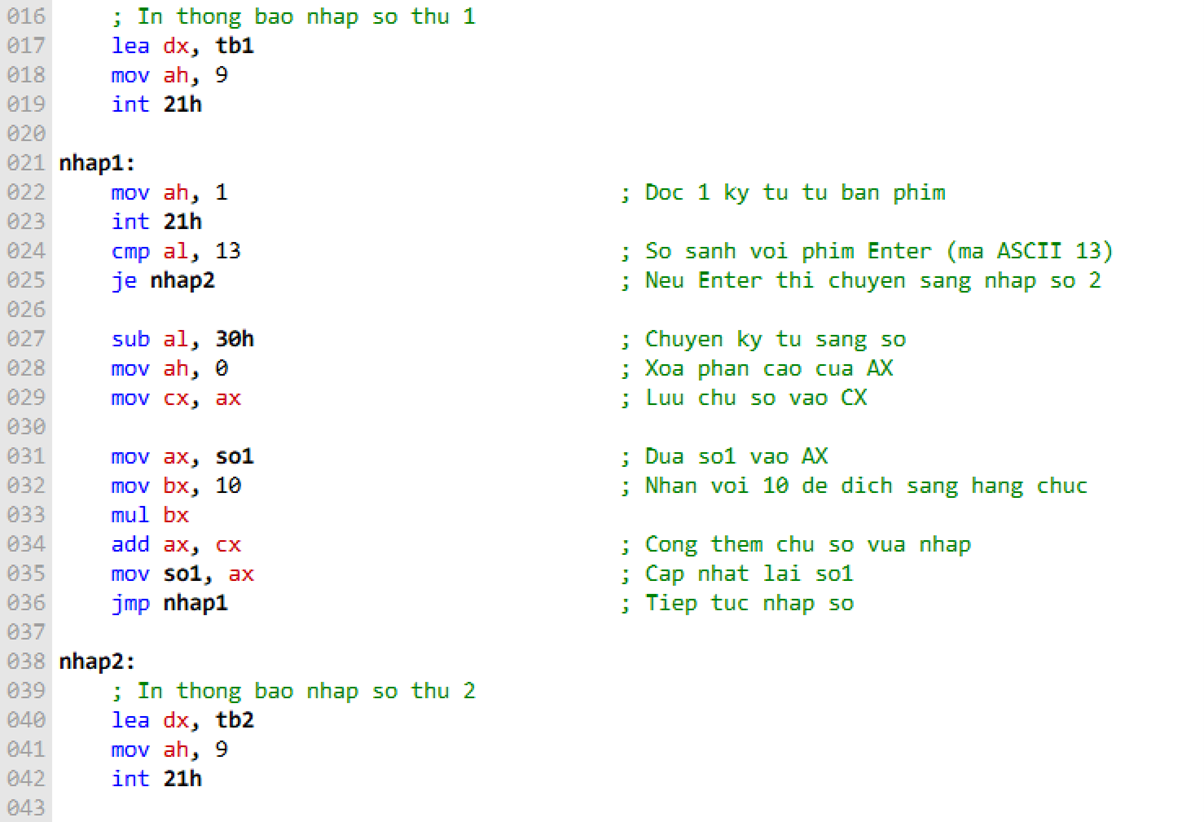
\includegraphics[width=0.9\textwidth]{Thái/Picture8.png}
\end{figure}


\begin{figure}[H]
    \centering
    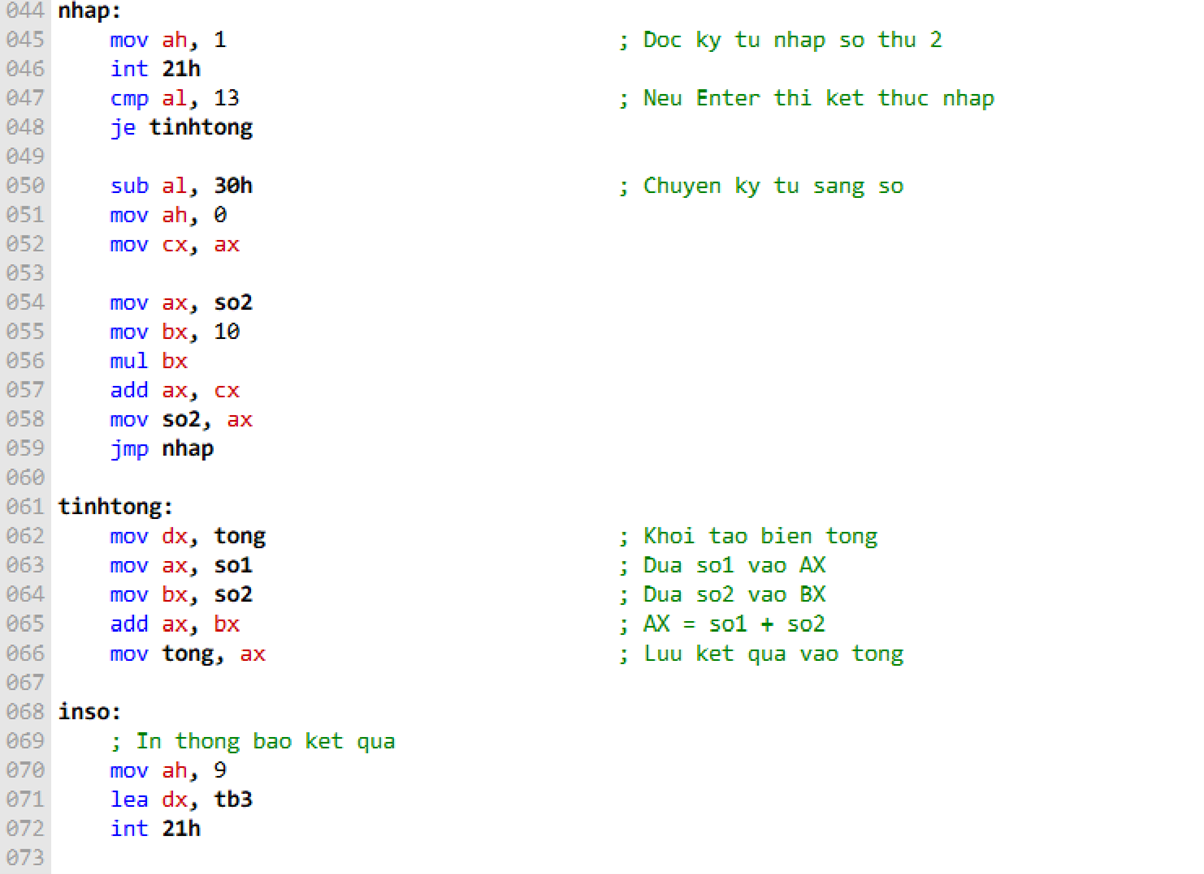
\includegraphics[width=0.9\textwidth]{Thái/Picture9.png}
     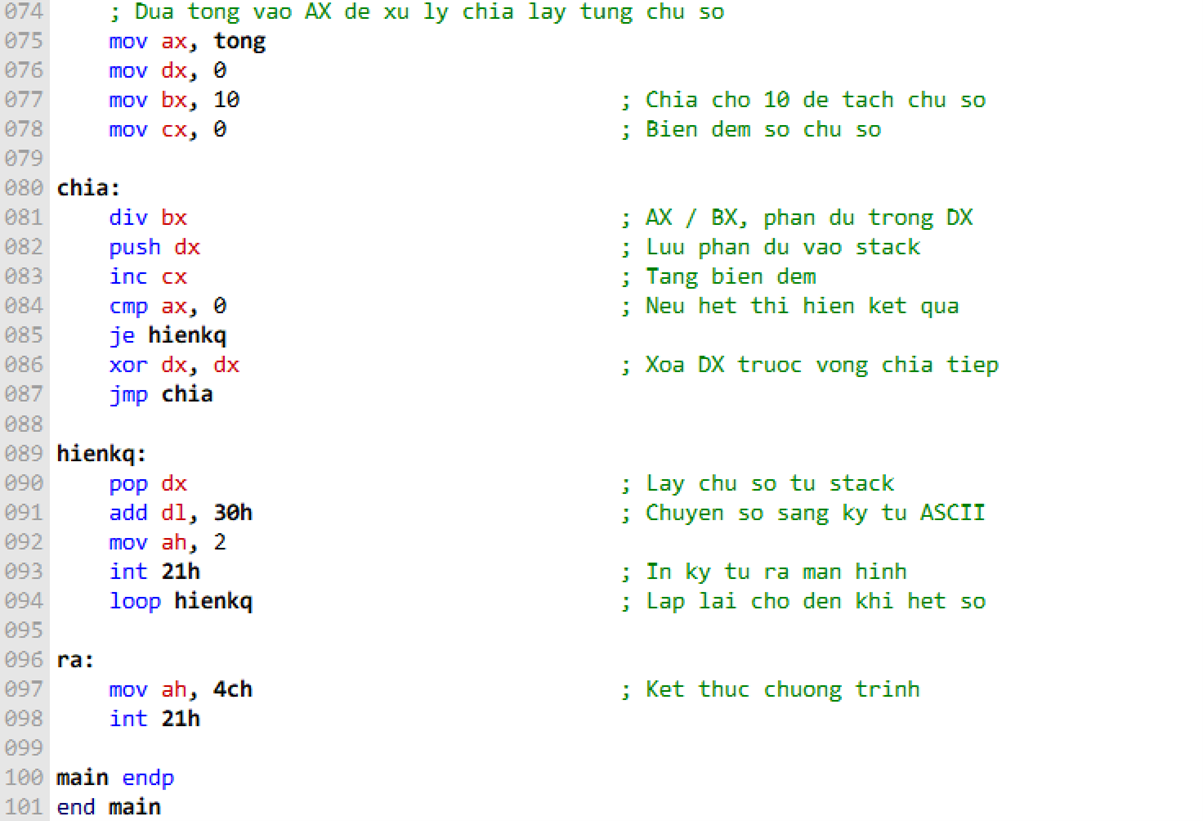
\includegraphics[width=0.9\textwidth]{Thái/Picture10.png}
    \caption{Mã nguồn in ra tổng 2 số theo kiểu word}
\end{figure}

\begin{figure}[H]
    \centering
      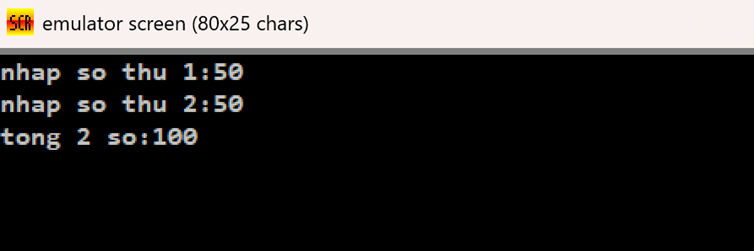
\includegraphics[width=0.9\textwidth]{Thái/Picture11.png}
    \caption{Giao diện in ra tổng 2 số theo kiểu word}
\end{figure}

\section{Bài tập của Vũ Quang Huy}

\subsection{Chuyển chuỗi ký tự thành dạng viết hoa và viết thường}
Chương trình hợp ngữ Assembly cho phép nhập 1 chuỗi ký tự, in ra màn hình chuỗi ký tự đó theo dạng viết hoa và viết thường.

\begin{figure}[H]
    \centering
    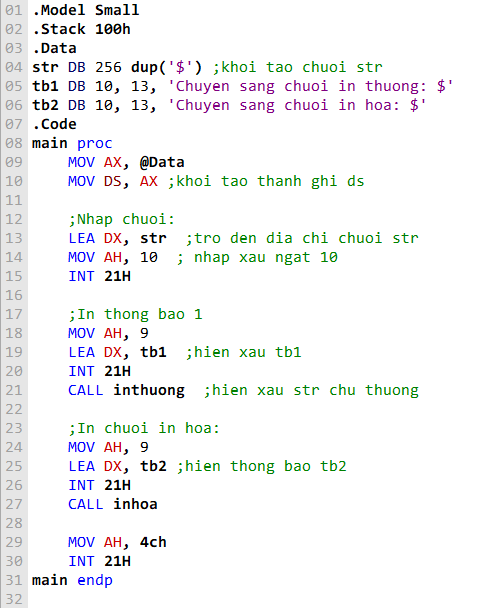
\includegraphics[width=0.8\textwidth]{Huy/1.5.1.png}
\end{figure}

\begin{figure}[H]
    \centering
    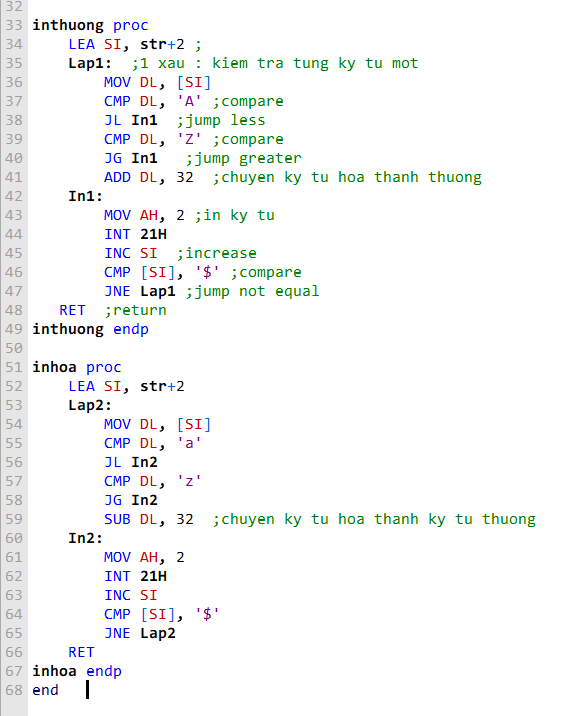
\includegraphics[width=0.8\textwidth]{Huy/1.5.2.png}
    \caption{Mã nguồn in ra chuỗi theo dạng viết hoa và viết thường}
\end{figure}

\begin{figure}[H]
    \centering
    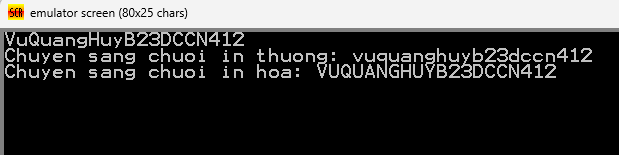
\includegraphics[width=0.8\textwidth]{Huy/1.5.3.png}
    \caption{Giao diện in ra chuỗi theo dạng viết hoa và viết thường}
\end{figure}

\subsection{In chuỗi ký tự theo thứ tự ngược lại}
Chương trình hợp ngữ Assembly cho phép nhập một chuỗi các ký tự kết thúc bởi ``\#'' và yêu cầu in ra màn hình chuỗi ký tự đó theo thứ tự ngược lại.

\begin{figure}[H]
    \centering
    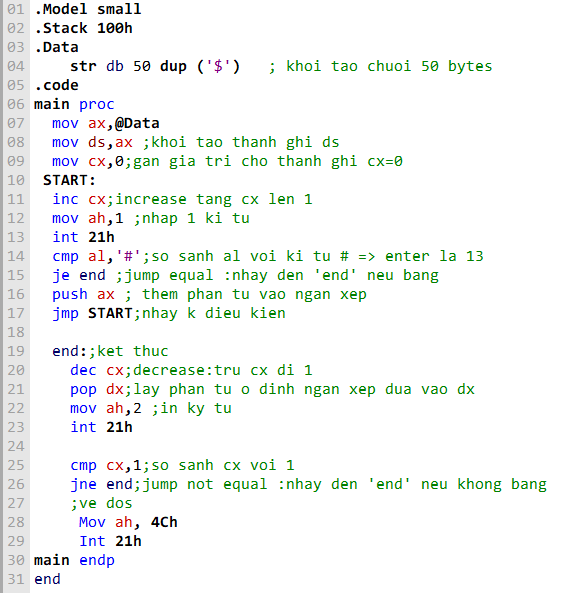
\includegraphics[width=0.8\textwidth]{Huy/1.6.1.png}
    \caption{Mã nguồn in ra chuỗi kết thúc bởi '\#' theo thứ tự ngược lại}
\end{figure}

\begin{figure}[H]
    \centering
     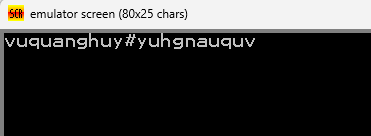
\includegraphics[width=0.8\textwidth]{Huy/1.6.2.png}
    \caption{Giao diện in ra chuỗi kết thúc bởi '\#' theo thứ tự ngược lại}
\end{figure}

\subsection{Tìm giá trị lớn nhất và nhỏ nhất của một mảng số}
Chương trình hợp ngữ Assembly tìm giá trị lớn nhất và nhỏ nhất của một mảng số.

\begin{figure}[H]
    \centering
     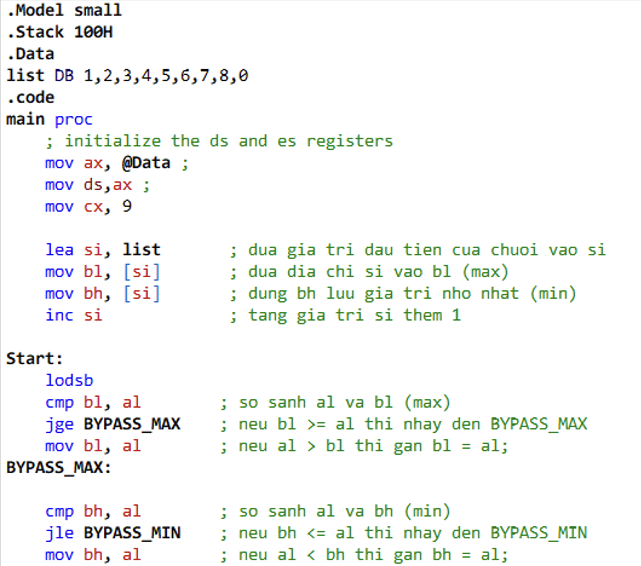
\includegraphics[width=0.8\textwidth]{Huy/1.11.1.png}
\end{figure}

\begin{figure}[H]
    \centering
     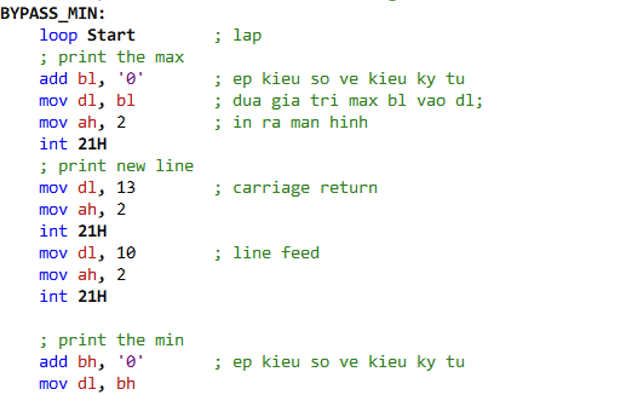
\includegraphics[width=0.8\textwidth]{Huy/1.11.2.png}
    \caption{Mã nguồn in ra giá trị lớn nhất và nhỏ nhất của mảng số}
\end{figure}

\begin{figure}[H]
    \centering
      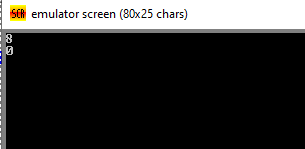
\includegraphics[width=0.8\textwidth]{Huy/1.11.3.png}
    \caption{Giao diện in ra giá trị lớn nhất và nhỏ nhất của mảng số}
\end{figure}

\section{Bài tập của Lê Huy Hải}

\subsection{Chuyển số từ hệ cơ số 10 sang hệ nhị phân}
Chương trình hợp ngữ Assembly chuyển một số từ hệ cơ số 10 sang hệ nhị phân.

\begin{figure}[H]
    \centering
    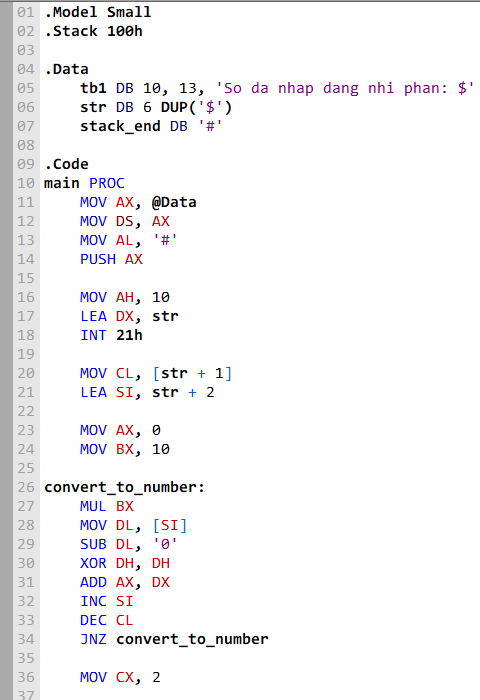
\includegraphics[width=0.8\textwidth]{Hải/Image_01.png}
\end{figure}

\begin{figure}[H]
    \centering
    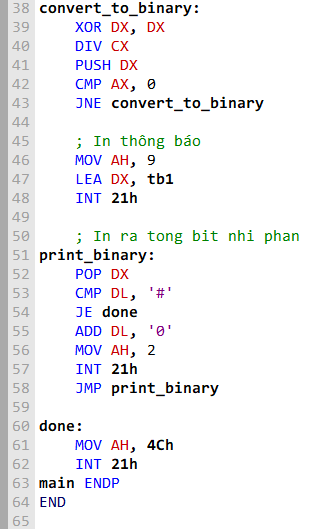
\includegraphics[width=0.8\textwidth]{Hải/Image_02.png}
    \caption{Mã nguồn chuyển số từ hệ cơ số 10 sang hệ nhị phân}
\end{figure}

\begin{figure}[H]
    \centering
     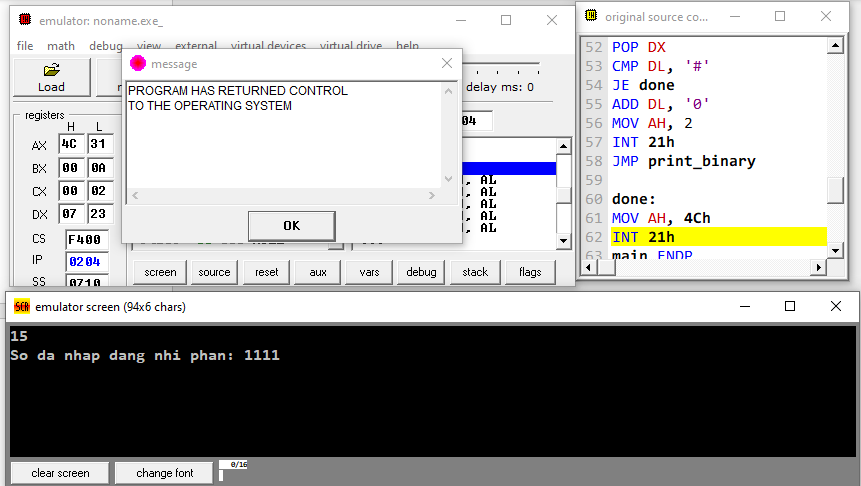
\includegraphics[width=0.8\textwidth]{Hải/Image_03.png}
    \caption{Kết quả in ra khi đã chuyển đổi sang hệ nhị phân}
\end{figure}

\subsection{Đếm chiều dài của một chuỗi ký tự}
Chương trình hợp ngữ Assembly yêu cầu đếm chiều dài của một chuỗi ký tự cho trước.

\begin{figure}[H]
    \centering
     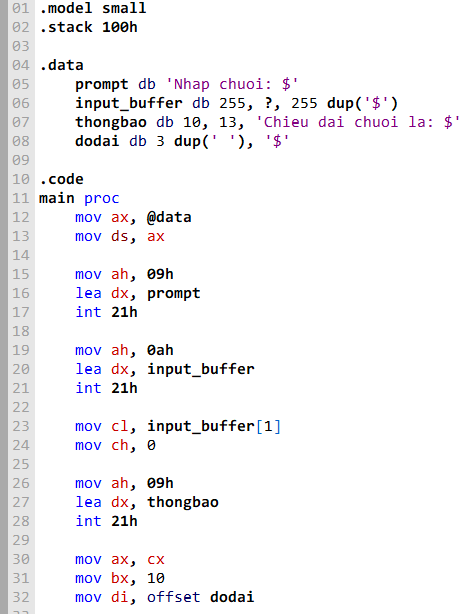
\includegraphics[width=0.8\textwidth]{Hải/Image_04.png}
\end{figure}


\begin{figure}[H]
    \centering
     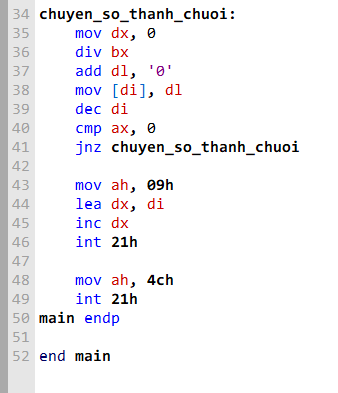
\includegraphics[width=0.8\textwidth]{Hải/Image_05.png}
    \caption{Mã Nguồn đếm chiều dài của xâu kí tự cho trước}
\end{figure}

\begin{figure}[H]
    \centering
     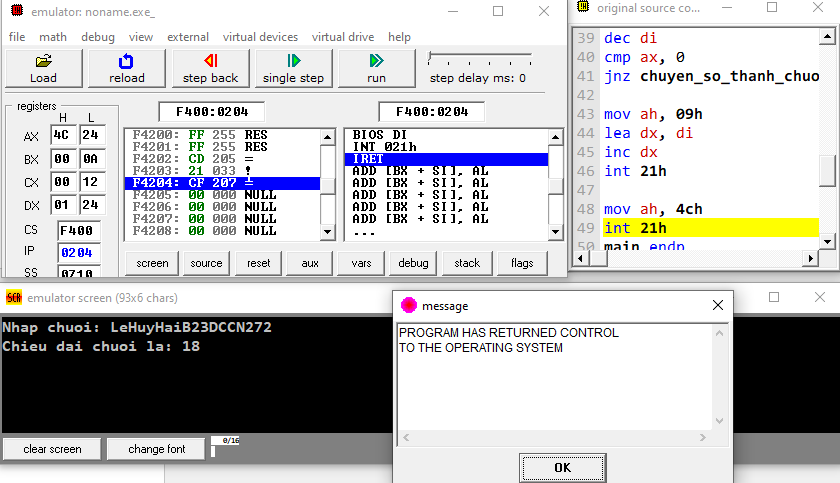
\includegraphics[width=0.8\textwidth]{Hải/Image_06.png}
    \caption{Kết quả in ra khi tính chiều dài của chuỗi}
\end{figure}

\subsection{Tính tổng các số}
Chương trình hợp ngữ Assembly cho phép nhập vào các số và in ra màn hình tổng của các số đó.

\begin{figure}[H]
    \centering
     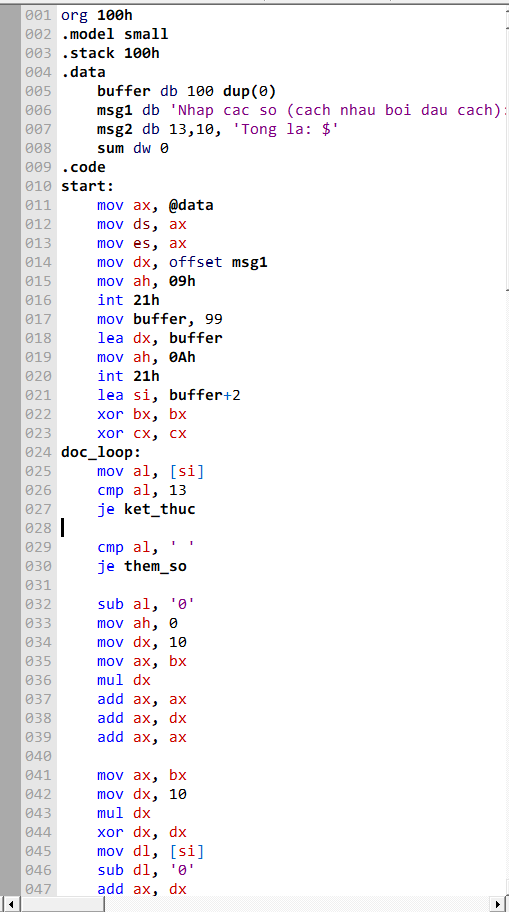
\includegraphics[width=0.7\textwidth]{Hải/Image_07.png}
\end{figure}

\begin{figure}[H]
    \centering
     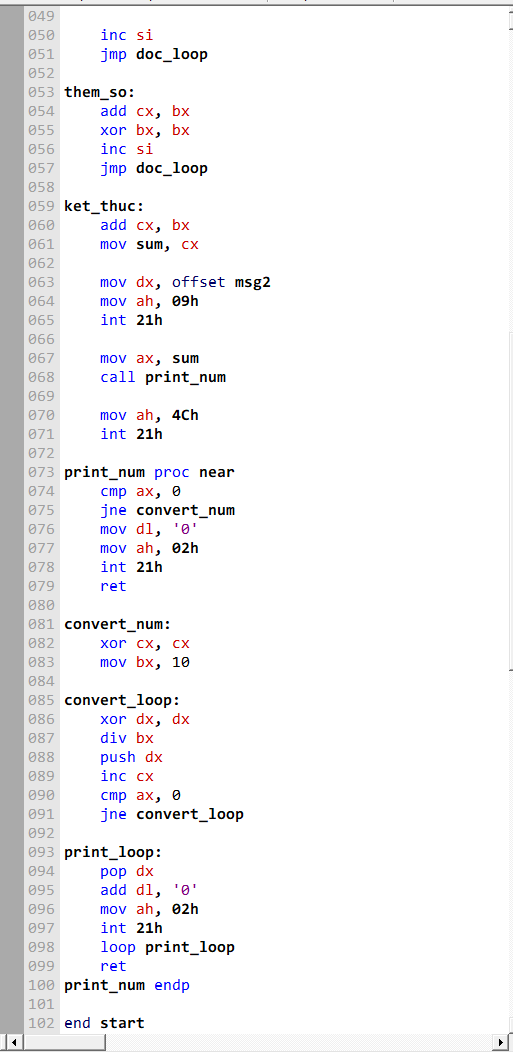
\includegraphics[width=0.7\textwidth]{Hải/Image_08.png}
    \caption{Mã nguồn in ra tổng các số cho trước}
\end{figure}

\begin{figure}[H]
    \centering
     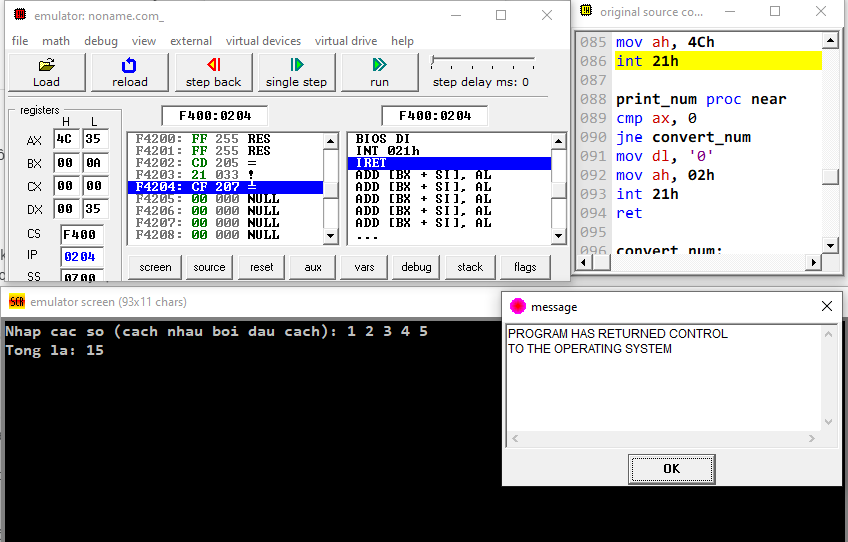
\includegraphics[width=0.8\textwidth]{Hải/Image_09.png}
    \caption{Kết quả in ra tổng của các số đã cho}
\end{figure}

\section{Bài tập của Hà Duy Khánh}

\subsection{Lời chào tiếng Anh \& tiếng Việt}
Chương trình hợp ngữ Assembly hiển thị lời chào bằng tiếng Anh và tiếng Việt.

\begin{figure}[H]
    \centering
     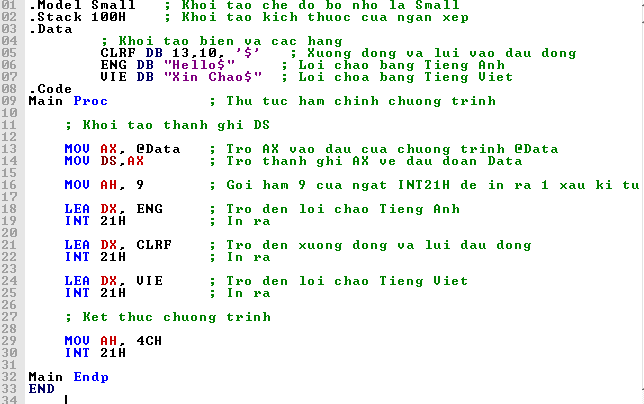
\includegraphics[width=0.8\textwidth]{Khánh/1.png}    
    \caption{Mã nguồn in ra lời chào bằng tiếng Việt và tiếng Anh}
\end{figure}

\begin{figure}[H]
    \centering
     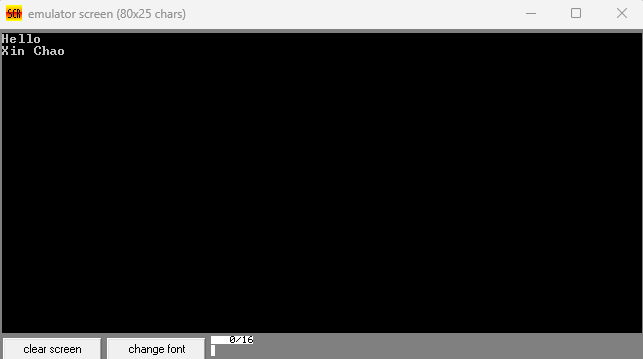
\includegraphics[width=0.8\textwidth]{Khánh/2.png}
    \caption{Kết quả in ra lời chào bằng tiếng Việt và tiếng Anh}
\end{figure}

\subsection{Nhập 1 ký tự và in ra}
Chương trình hợp ngữ Assembly nhập một ký tự và hiển thị ra màn hình.

\begin{figure}[H]
    \centering
     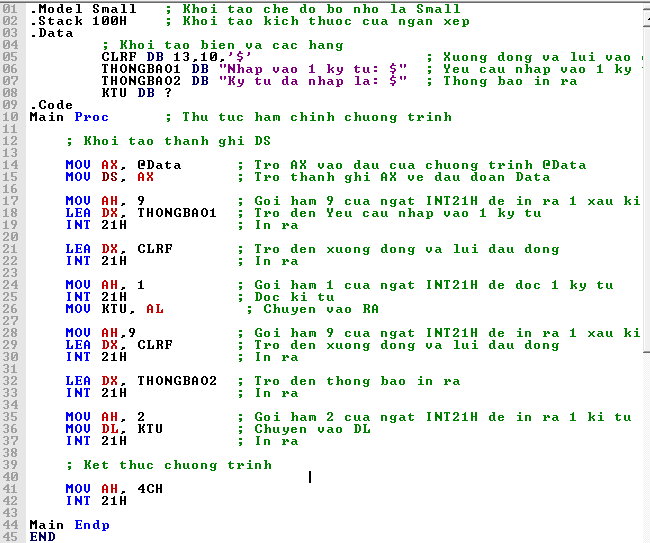
\includegraphics[width=0.8\textwidth]{Khánh/3.png}
    \caption{Mã nguồn nhập 1 ký tự và hiện thị ra màn hình}
\end{figure}

\begin{figure}[H]
    \centering
     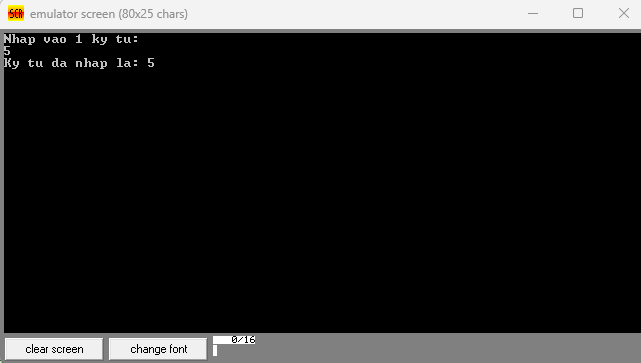
\includegraphics[width=0.8\textwidth]{Khánh/4.png}
    \caption{Giao diện hiện thị 1 ký tự ra màn hình}
\end{figure}

\subsection{Tính giai thừa}
Chương trình hợp ngữ Assembly tính giai thừa của một số.

\begin{figure}[H]
    \centering
     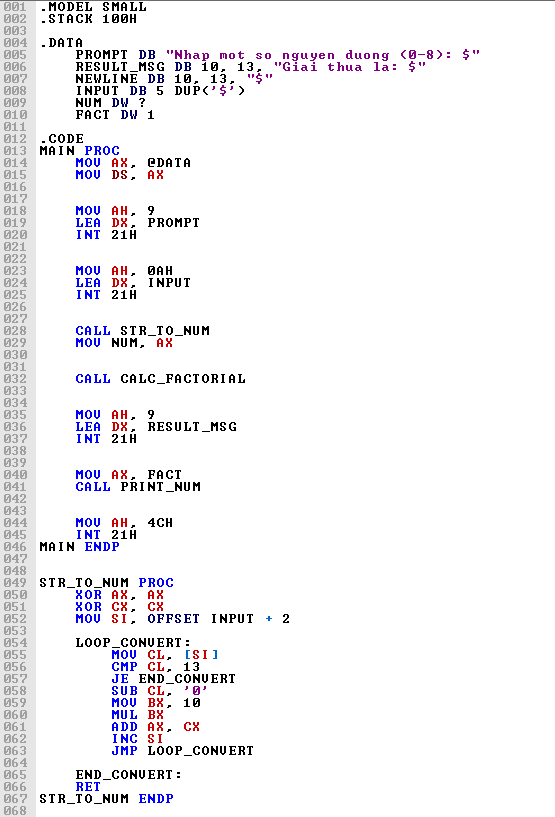
\includegraphics[width=0.8\textwidth]{Khánh/5.png}
\end{figure}
\begin{figure}[H]
    \centering
     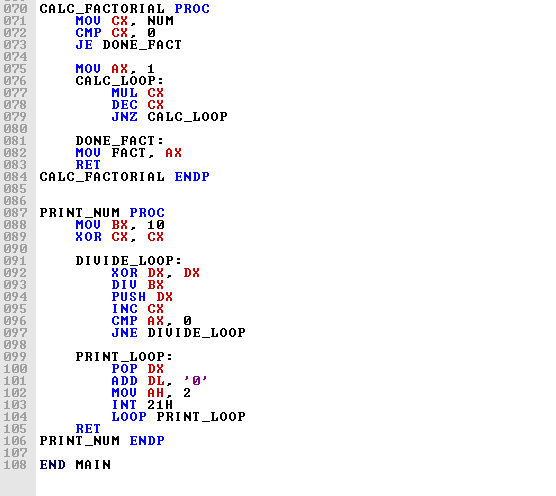
\includegraphics[width=0.8\textwidth]{Khánh/6.png}
    \caption{Mã nguồn tính giai thừa của 1 số}
\end{figure}
\begin{figure}[H]
    \centering
     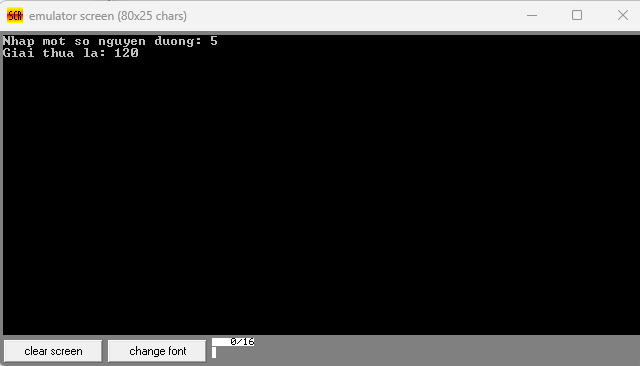
\includegraphics[width=0.8\textwidth]{Khánh/7.png}
    \caption{Kết quả phép tính giai thừa của 1 số}
\end{figure}

\chapter{Phân tích khảo sát hệ thống bộ nhớ}
\label{ch:memory_analysis}

\section{Nguyễn Trường Thái}

\subsection{Khảo sát cấu hình máy}
Khảo sát cấu hình của máy và hệ thống bộ nhớ của máy đang sử dụng (Bộ nhớ trong: ROM, RAM, Cache System,..) được thực hiện bằng phần mềm CPU-Z.



\subsubsection{CPU}
\begin{figure}[H]
    \centering
    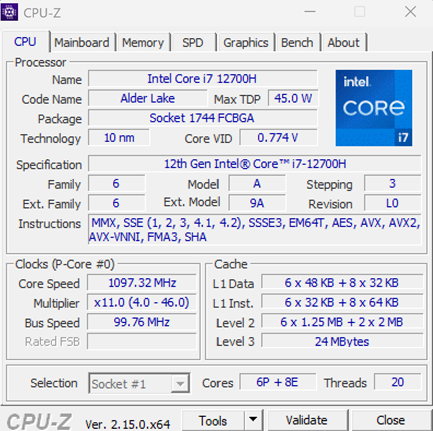
\includegraphics[width=0.8\textwidth]{Thái/Picture12.png}
    \caption{Intel Core i7-12700H – 14 Nhân – 20 Luồng}
\end{figure}


\subsubsection{Cache}
\begin{figure}[H]
    \centering
    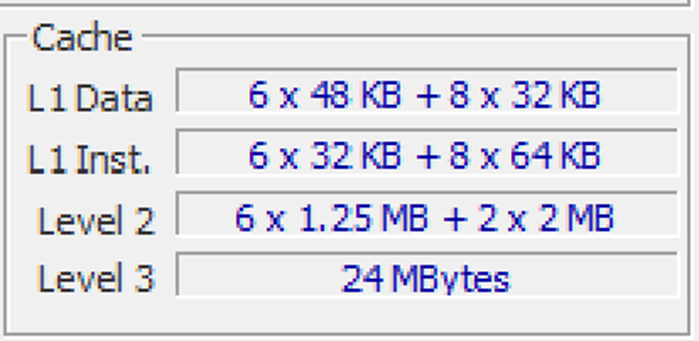
\includegraphics[width=0.8\textwidth]{Thái/Picture13.png}
    \caption{Hệ thống cache của máy tính bao gồm các cấp L1, L2, và L3.}
\end{figure}


\subsubsection{RAM}
\begin{figure}[H]
    \centering
    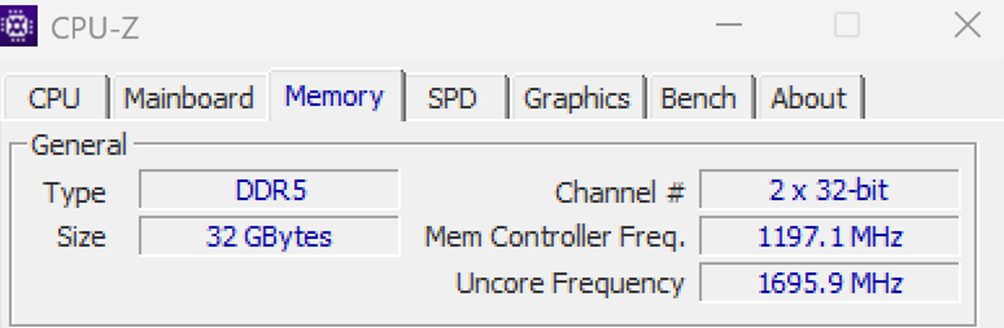
\includegraphics[width=0.8\textwidth]{Thái/Picture14.png}
    \caption{32Gb.}
\end{figure}

\subsubsection{Bộ nhớ ngoài}
\begin{figure}[H]
    \centering
    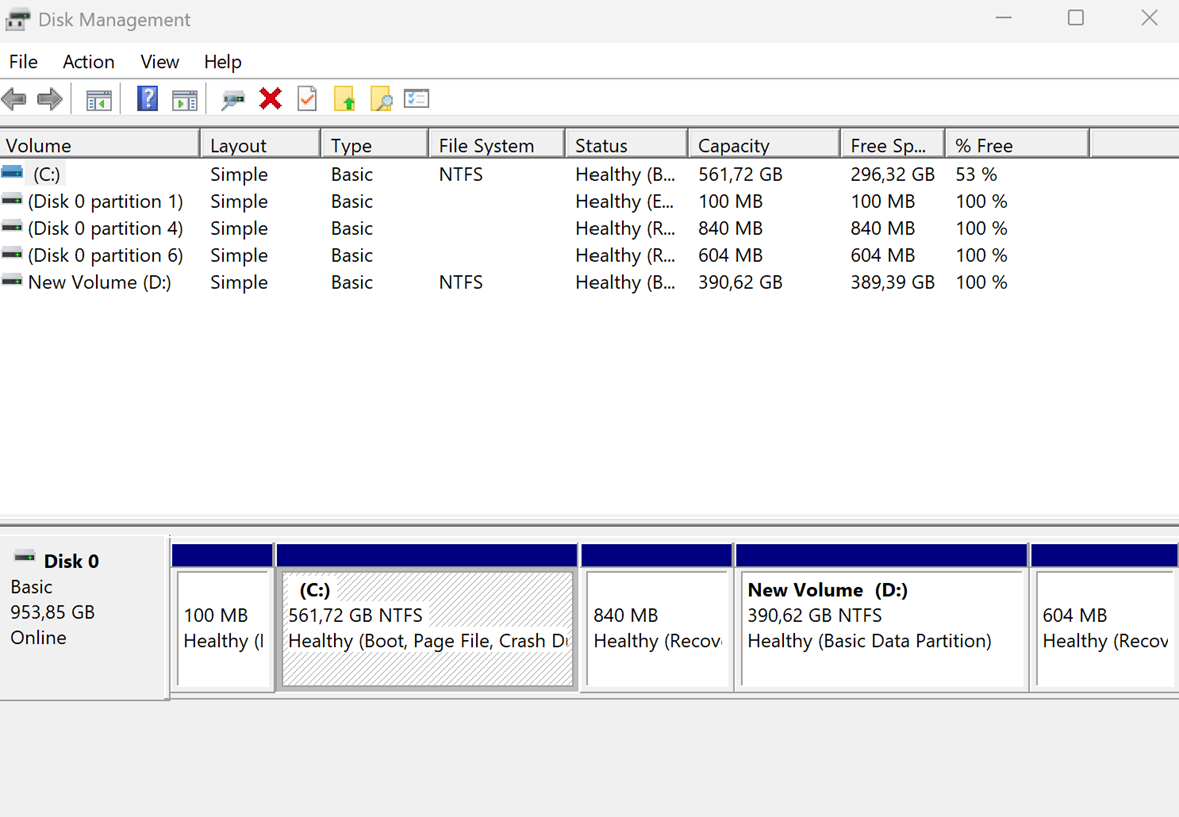
\includegraphics[width=0.9\textwidth]{Thái/Picture15.png}
\end{figure}


\subsubsection{Các thiết bị vào ra}
\begin{figure}[H]
    \centering
     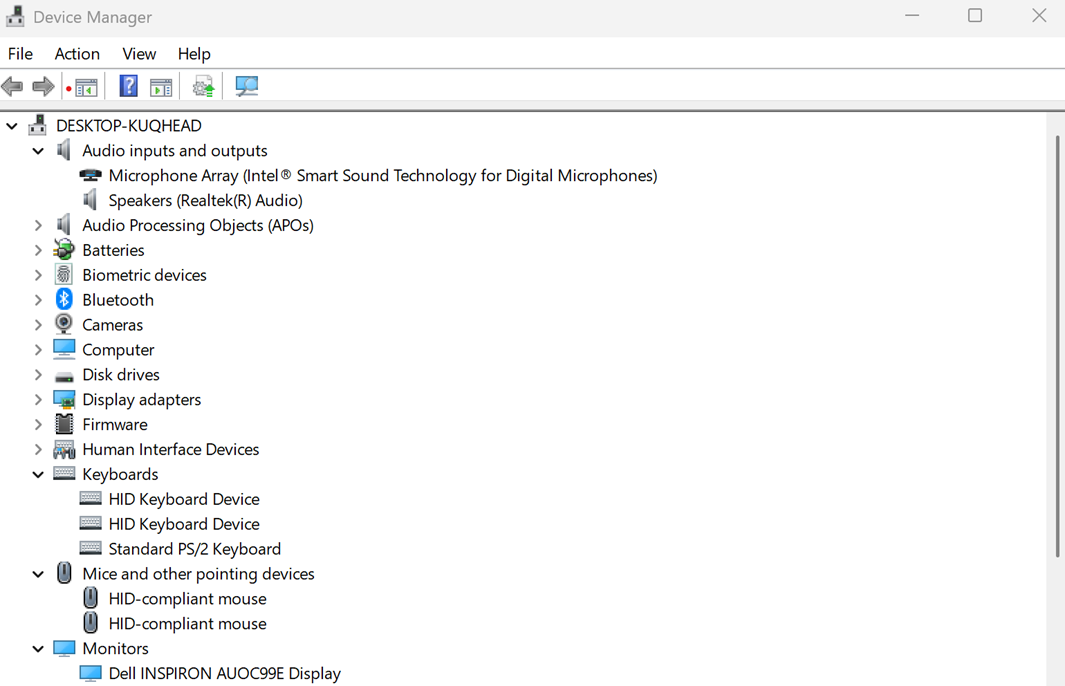
\includegraphics[width=1\textwidth]{Thái/Picture16.png}
     \caption{ Bao gồm bàn phím, chuột, màn hình, và các cổng kết nối.}
\end{figure}




\subsection{Khảo sát nội dung các thanh ghi}


\subsubsection{Giải thích nội dung các thanh ghi}
Dùng công cụ Debug khảo sát nội dung các thanh ghi IP, DS, ES, SS, CS, BP, SP

\begin{itemize}
    \item Công cụ sử dụng: emu8086 microprocessor emulator
    \item Các bước thực hiện:
    \item Mở file .asm bằng phần mềm trên
    \item Chọn emulate trên thanh công cụ rồi chọn nút debug nằm cuối của cửa sổ vừa mở ra
    \item Chạy Single step để xem kết quả debug từng mã lệnh từ đầu đến cuối
\end{itemize}

\begin{figure}[H]
    \centering
    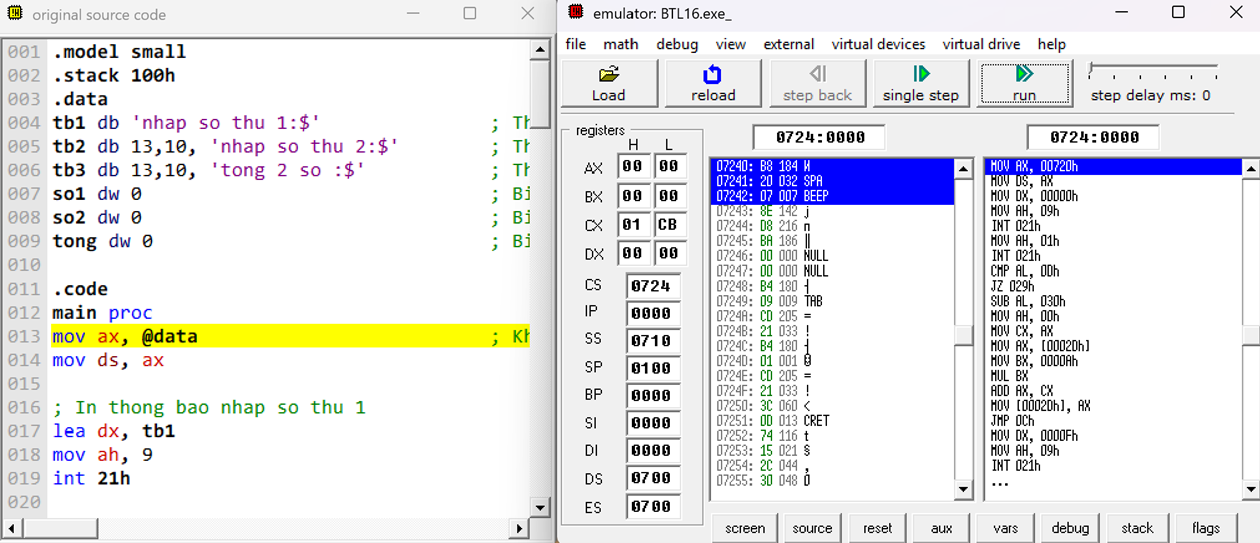
\includegraphics[width=1\textwidth]{Thái/Picture17.png}
\end{figure}

\begin{figure}[H]
    \centering
    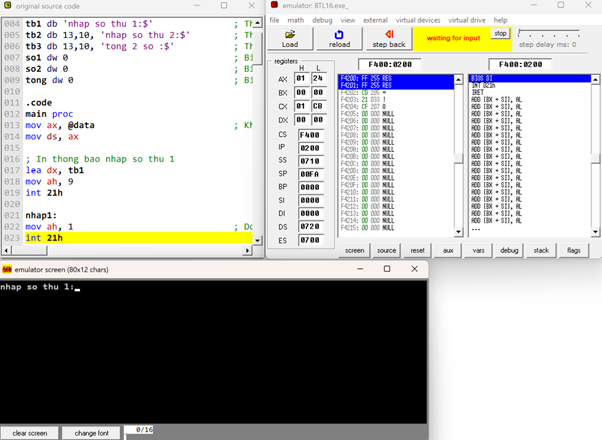
\includegraphics[width=1\textwidth]{Thái/Picture18.png}
\end{figure}

\begin{figure}[H]
    \centering
    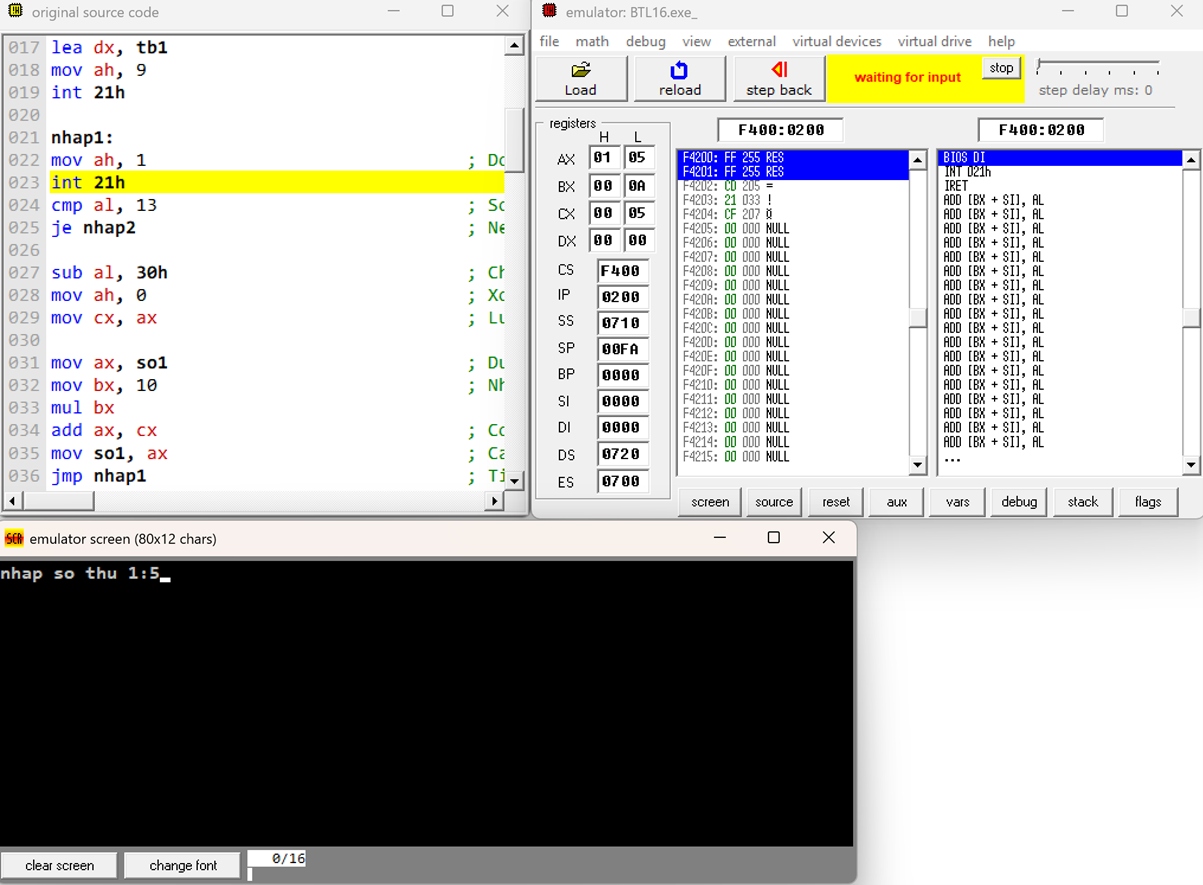
\includegraphics[width=0.95\textwidth]{Thái/Picture19.png}
\end{figure}

\begin{figure}[H]
    \centering
    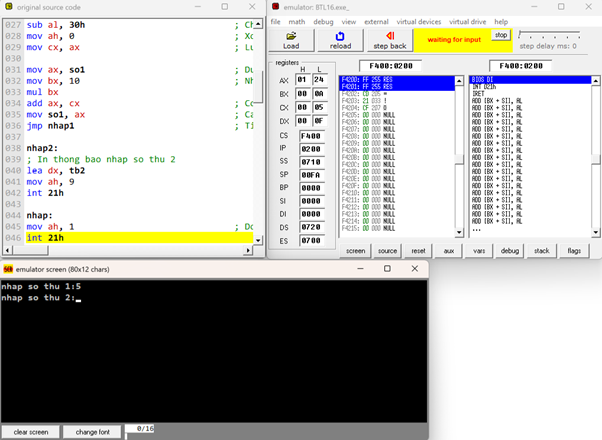
\includegraphics[width=0.95\textwidth]{Thái/Picture20.png}
\end{figure}

\begin{figure}[H]
    \centering
    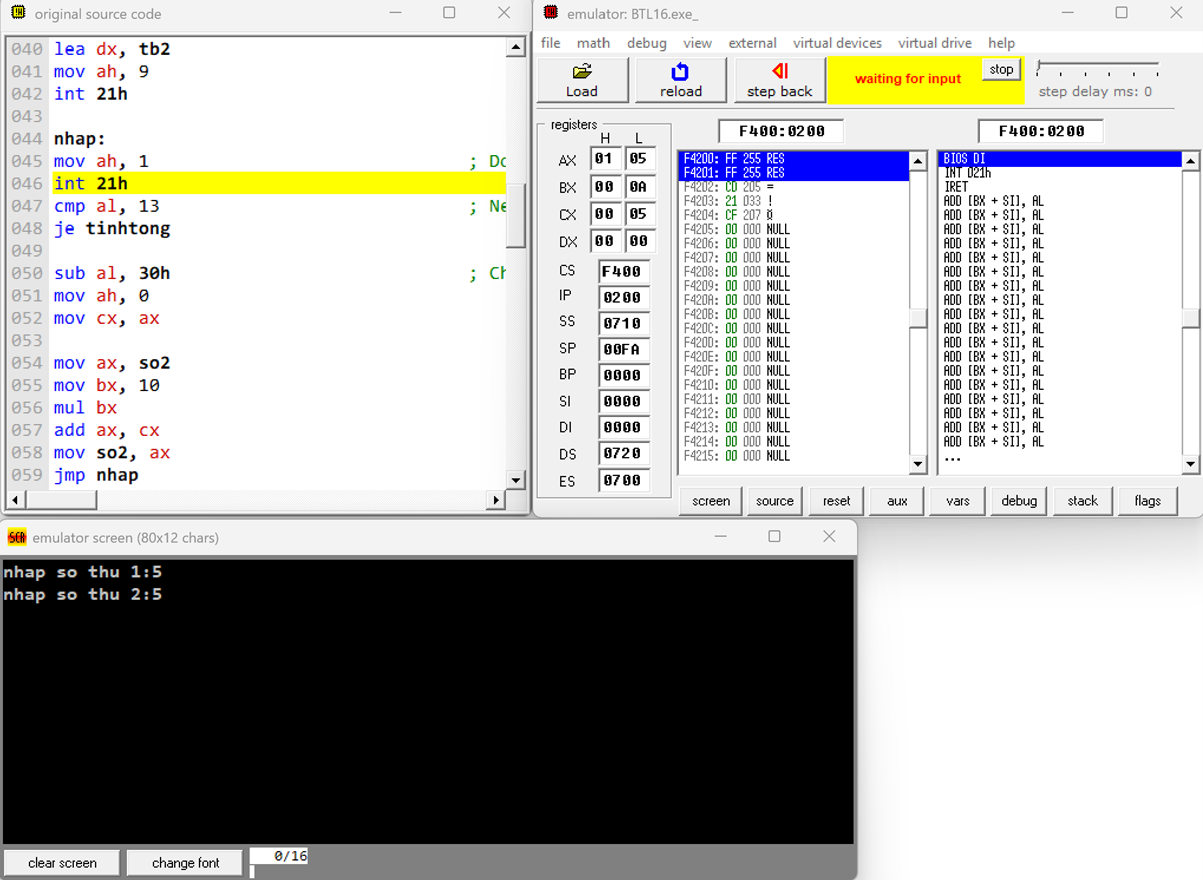
\includegraphics[width=0.95\textwidth]{Thái/Picture21.png}
\end{figure}

\begin{figure}[H]
    \centering
    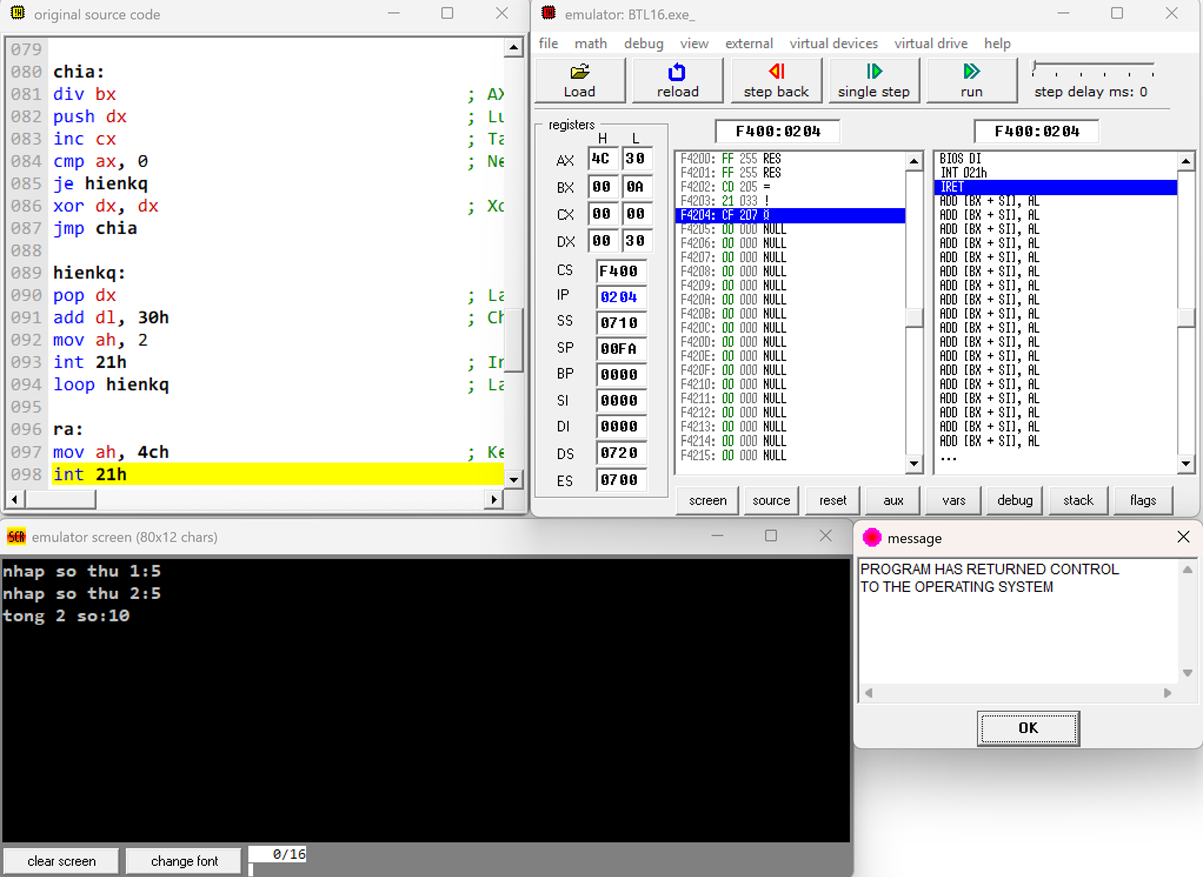
\includegraphics[width=0.95\textwidth]{Thái/Picture22.png}
\end{figure}


\subsection{Giải thích nội dung các thanh ghi}
Khi chương trình bắt đầu chạy, hệ điều hành tự động khởi tạo các thanh ghi, vùng nhớ và cấp phát không gian địa chỉ cho chương trình. Tương ứng với các câu lệnh trong mã nguồn, nội dung các thanh ghi có thể thay đổi hoặc không.

\subsubsection{IP (Instruction Pointer)}
\begin{itemize}
    \item IP là thanh ghi trỏ đến địa chỉ của lệnh tiếp theo sẽ được thực thi trong mã máy.
    \item Khi một chương trình được thực thi, IP được cập nhật để trỏ đến lệnh tiếp theo trong mã nguồn. Điều này giúp CPU biết lệnh nào sẽ được thực thi tiếp theo.
\end{itemize}

\subsubsection{DS (Data Segment) và SI (Source Index)}
\begin{itemize}
    \item DS là thanh ghi chỉ đến phân đoạn dữ liệu, nơi dữ liệu chương trình được lưu trữ.
    \item SI thường được sử dụng trong các phép toán dữ liệu và là một trong các thanh ghi chỉ địa chỉ.
    \item Khi chương trình yêu cầu truy cập dữ liệu từ bộ nhớ, DS và SI thường được sử dụng để xác định vị trí của dữ liệu trong bộ nhớ.
\end{itemize}

\subsubsection{SS (Stack Segment) và BP (Base Pointer)}
\begin{itemize}
    \item SS là thanh ghi chỉ đến phân đoạn ngăn xếp (stack segment), nơi các giá trị cục bộ và địa chỉ của các hàm được lưu trữ.
    \item BP thường được sử dụng để trỏ đến địa chỉ cơ sở của ngăn xếp (base of stack).
    \item Ngăn xếp được sử dụng để lưu trữ các giá trị trung gian và địa chỉ trả về từ các hàm con (subroutines) trong quá trình thực thi chương trình.
\end{itemize}

\subsubsection{SP (Stack Pointer)}
\begin{itemize}
    \item SP là thanh ghi chỉ đến đỉnh của ngăn xếp (top of stack).
    \item Khi dữ liệu được đẩy (push) hoặc rút (pop) ra khỏi ngăn xếp, SP sẽ thay đổi để chỉ đến vị trí mới nhất trong ngăn xếp.
    \item SP cũng được sử dụng để cấp phát không gian mới cho dữ liệu trong ngăn xếp.
\end{itemize}

\subsection{Cơ chế quản lý bộ nhớ}

Cụ thể, trong trường hợp của đoạn chương trình chuyển xâu ký tự thành xâu in hoa và in thường tương ứng, ta có cơ chế quản lý bộ nhớ như sau:

\subsubsection{Khởi tạo bộ nhớ}
\begin{itemize}
    \item Khi chương trình bắt đầu, HĐH sẽ cấp phát các đoạn mã (code), dữ liệu (data), và ngăn xếp (stack) cho chương trình.
    \item Đoạn mã chứa các lệnh chương trình, đoạn dữ liệu chứa các biến, và đoạn ngăn xếp dùng để lưu trữ dữ liệu tạm thời.
\end{itemize}

\subsubsection{Phân đoạn bộ nhớ}
\begin{itemize}
    \item CS (Code Segment) trỏ tới đoạn mã của chương trình.
    \item DS (Data Segment) trỏ tới đoạn dữ liệu của chương trình.
    \item SS (Stack Segment) trỏ tới đoạn ngăn xếp của chương trình.
\end{itemize}

\subsubsection{Quản lý ngăn xếp}
\begin{itemize}
    \item Ngăn xếp được sử dụng để lưu trữ tạm thời dữ liệu và địa chỉ trả về khi gọi hàm.
    \item SP được khởi tạo với giá trị từ khai báo .Stack 100H, nghĩa là kích thước ngăn xếp là 256 byte.
\end{itemize}



\subsubsection{Diễn giải mã nguồn và ảnh hưởng đến thanh ghi}
\begin{itemize}
    \item \textbf{Khởi tạo đoạn dữ liệu:} 
\begin{figure}[H]
    \centering
    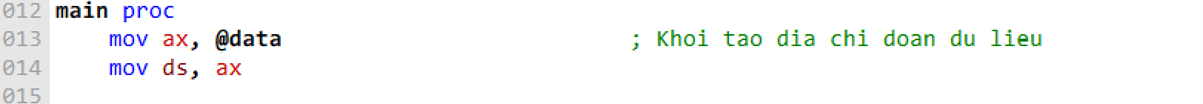
\includegraphics[width=1\textwidth]{Thái/Picture23.png}
\end{figure}
    DS trỏ tới đoạn dữ liệu. Thanh ghi AX được dùng làm trung gian để nạp địa chỉ đoạn dữ liệu vào DS.
    
    \item \textbf{Hiển thị thông báo và đọc chuỗi ký tự:} 
\begin{figure}[H]
    \centering
    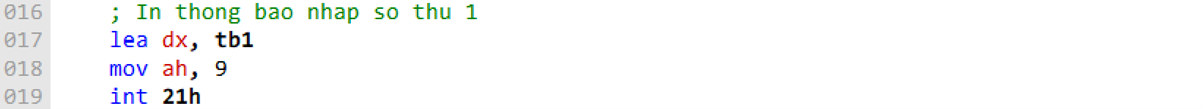
\includegraphics[width=1\textwidth]{Thái/Picture24.png}
\end{figure}
    AH = 9 gọi hàm in chuỗi của ngắt 21h; DX chứa địa chỉ chuỗi cần in.

    \item \textbf{Nhập số thứ nhất từng chữ số và ghép thành số nguyên:} 
\begin{figure}[H]
    \centering
    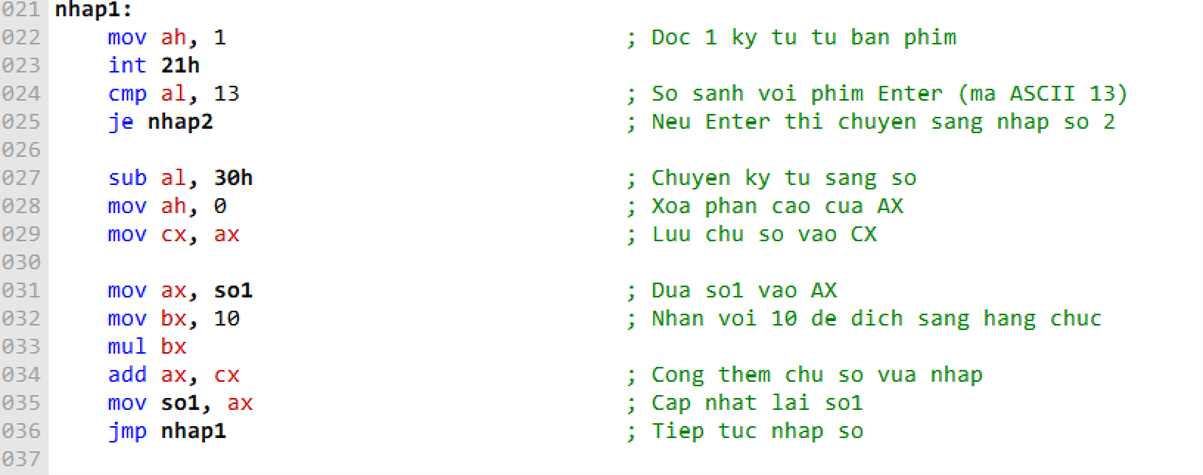
\includegraphics[width=1\textwidth]{Thái/Picture25.png}
\end{figure}    
    AH = 1 để đọc từng ký tự. Nếu AL = 13 (Enter), nhảy sang nhãn \texttt{nhap2}. Ký tự nhập được chuyển từ ASCII sang số, sau đó: \\
    so1 = so1 × 10 + chữ số mới.

    \item \textbf{Hiển thị thông báo nhập số thứ hai và nhập tương tự:} 
\begin{figure}[H]
    \centering
    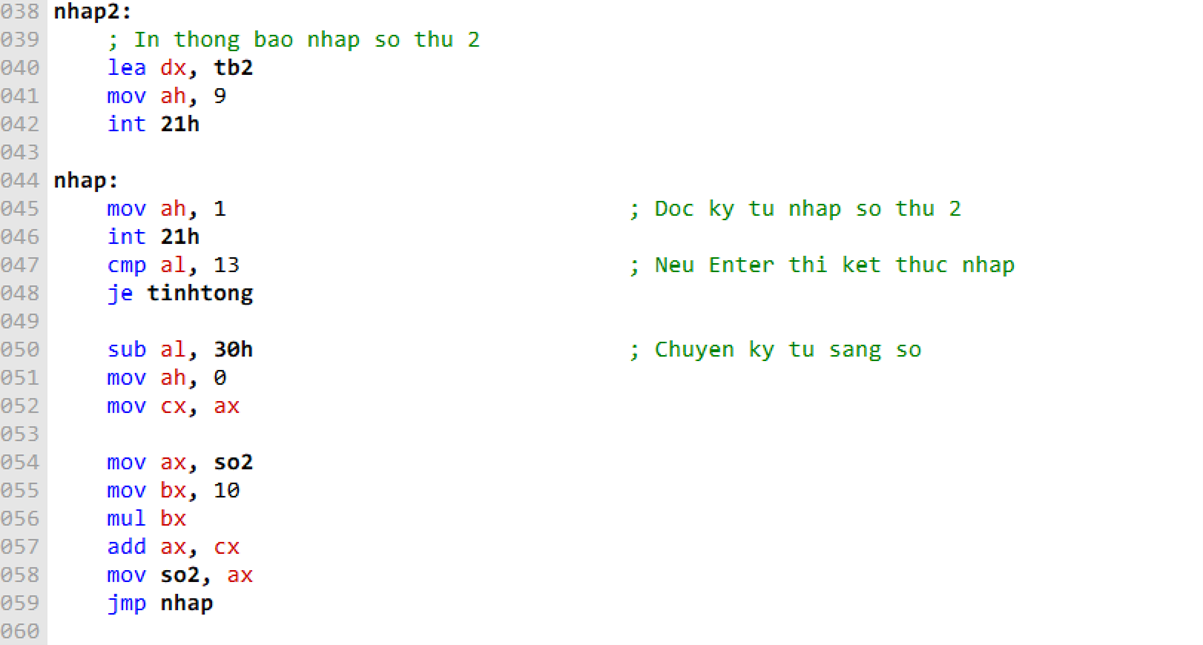
\includegraphics[width=1\textwidth]{Thái/Picture26.png}
\end{figure}
    In chuỗi thông báo với AH = 9, sau đó đọc từng ký tự bằng AH = 1. Nếu nhấn Enter thì nhảy đến nhãn \texttt{tinhtong}. \\
    so2 = so2 × 10 + chữ số mới (tương tự như so1).

\item \textbf{Tính tổng hai số, tách chữ số và in kết quả:}
\begin{figure}[H]
    \centering
    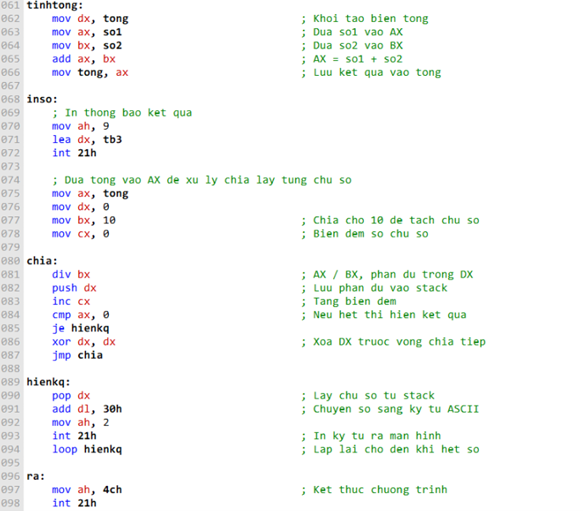
\includegraphics[width=1\textwidth]{Thái/Picture27.png}
\end{figure}
         Tính tổng: 
        \texttt{MOV AX, so1}, \texttt{MOV BX, so2}, \texttt{ADD AX, BX}, \texttt{MOV tong, AX} 
        
         In thông báo: 
        \texttt{MOV AH,9}, \texttt{LEA DX, tb3}, \texttt{INT 21h} 
        
        Chuẩn bị chia tách chữ số: 
        \texttt{MOV AX, tong}, \texttt{MOV DX,0}, \texttt{MOV BX,10}, \texttt{MOV CX,0} 
        
         \textbf{Vòng lặp chia (chia lấy chữ số, lưu stack):}
        \begin{itemize}
            \item \texttt{DIV BX}: Chia AX cho 10 → dư (chữ số) vào DX
            \item \texttt{PUSH DX}: Lưu chữ số lên stack (đảo ngược)
            \item \texttt{INC CX}: Tăng đếm chữ số
            \item \texttt{CMP AX,0 + JE hienkq}: Nếu AX=0 thì sang vòng in kết quả
            \item \texttt{XOR DX,DX}, \texttt{JMP chia}: Xóa DX và tiếp tục vòng chia
        \end{itemize}
        
         \textbf{Vòng lặp hienkq (lấy và in chữ số):}
        \begin{itemize}
            \item \texttt{POP DX}, \texttt{ADD DL,30h}: Lấy số và chuyển sang ASCII
            \item \texttt{MOV AH,2}, \texttt{INT 21h}: In ra màn hình
            \item \texttt{LOOP hienkq}: Lặp lại đến khi CX = 0
        \end{itemize}

         \textbf{Kết thúc chương trình:} \\
        \texttt{MOV AH,4Ch}, \texttt{INT 21h}
    
    
\end{itemize}


\section{Vũ Quang Huy}

\subsection{Khảo sát cấu hình máy}
Khảo sát cấu hình của máy và hệ thống bộ nhớ của máy đang sử dụng (Bộ nhớ trong: ROM, RAM, Cache System,..) được thực hiện bằng phần mềm CPU-Z.

\subsubsection{CPU}
\begin{figure}[H]
    \centering
    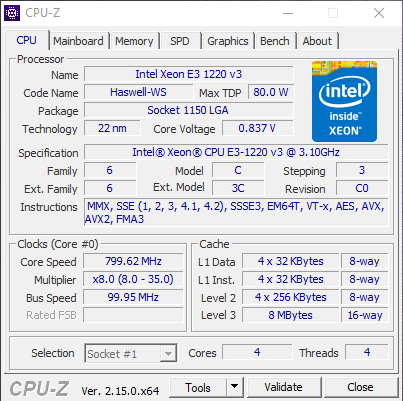
\includegraphics[width=0.9\textwidth]{Huy/2.1.1.png}
    \caption{Intel Xeon E3 1220 v3 - 4 Nhân - 4 Luồng.}
\end{figure}

\subsubsection{Cache}
\begin{figure}[H]
    \centering
    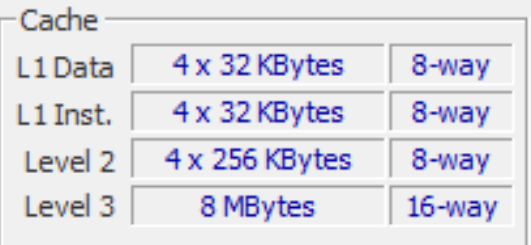
\includegraphics[width=0.9\textwidth]{Huy/2.1.2.png}
    \caption{Hệ thống cache của máy tính bao gồm các cấp L1, L2, và L3.}
\end{figure}

\subsubsection{RAM}
\begin{figure}[H]
    \centering
    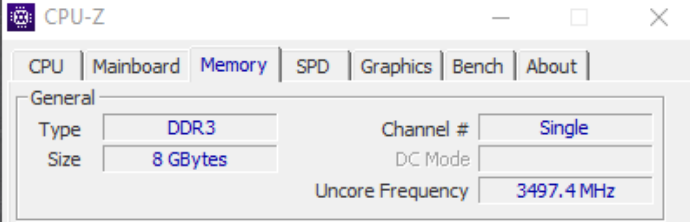
\includegraphics[width=0.9\textwidth]{Huy/2.1.3.png}
    \caption{8Gb.}
\end{figure}


\subsubsection{Bộ nhớ ngoài}
\begin{figure}[H]
    \centering
    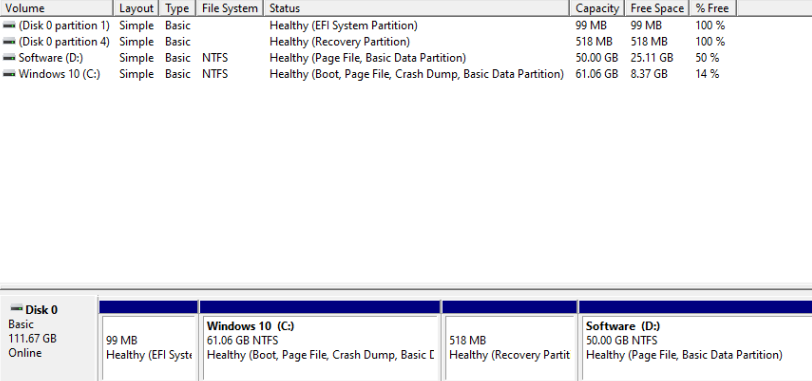
\includegraphics[width=1\textwidth]{Huy/2.1.4.png}
\end{figure}


\subsubsection{Các thiết bị vào ra}
\begin{figure}[H]
    \centering
    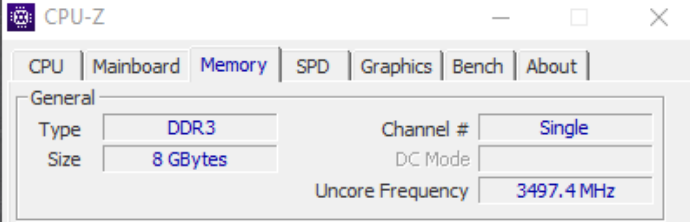
\includegraphics[width=0.9\textwidth]{Huy/2.1.3.png}
    \caption{Bao gồm bàn phím, chuột, màn hình, và các cổng kết nối.}
\end{figure}


\subsection{Khảo sát nội dung các thanh ghi}


\subsubsection{Giải thích nội dung các thanh ghi}
Dùng công cụ Debug khảo sát nội dung các thanh ghi IP, DS, ES, SS, CS, BP, SP

\begin{itemize}
    \item Công cụ sử dụng: emu8086 microprocessor emulator
    \item Các bước thực hiện:
    \item Mở file .asm bằng phần mềm trên
    \item Chọn emulate trên thanh công cụ rồi chọn nút debug nằm cuối của cửa sổ vừa mở ra
    \item Chạy Single step để xem kết quả debug từng mã lệnh từ đầu đến cuối
\end{itemize}

\begin{figure}[H]
    \centering
    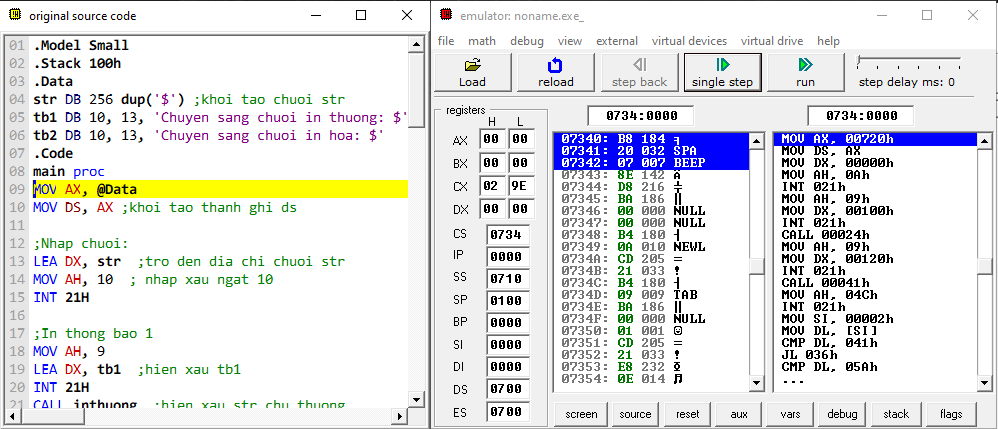
\includegraphics[width=1\textwidth]{Huy/2.2.1.png}
\end{figure}

\begin{figure}[H]
    \centering
    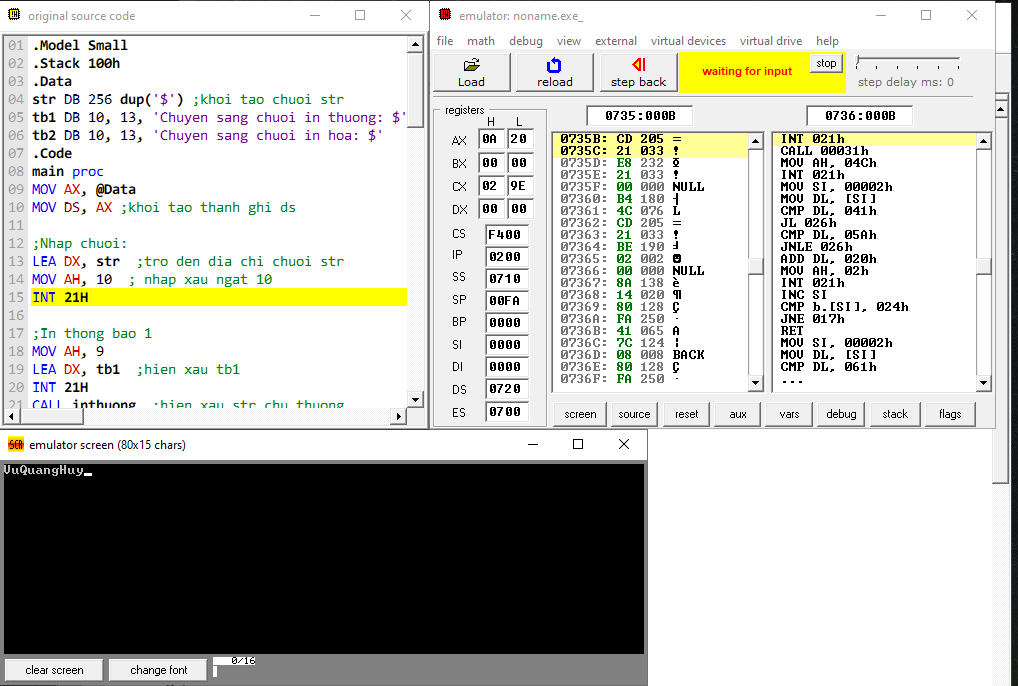
\includegraphics[width=1\textwidth]{Huy/2.2.2.png}
\end{figure}

\begin{figure}[H]
    \centering
    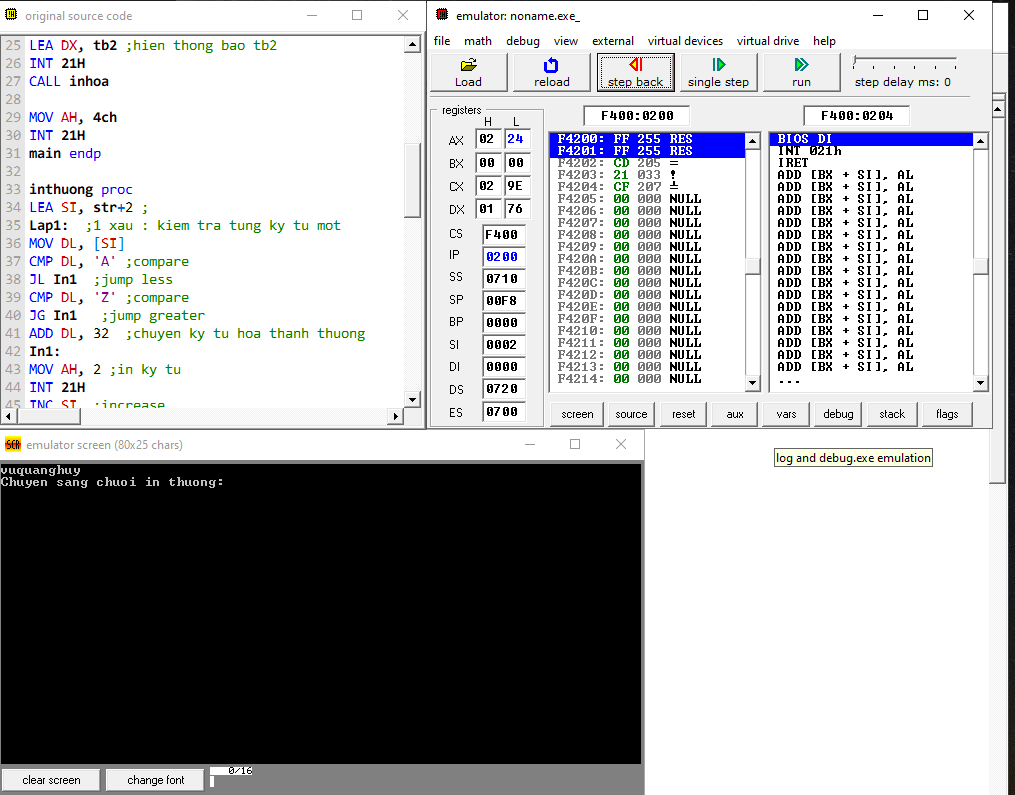
\includegraphics[width=0.9\textwidth]{Huy/2.2.3.png}
\end{figure}

\begin{figure}[H]
    \centering
    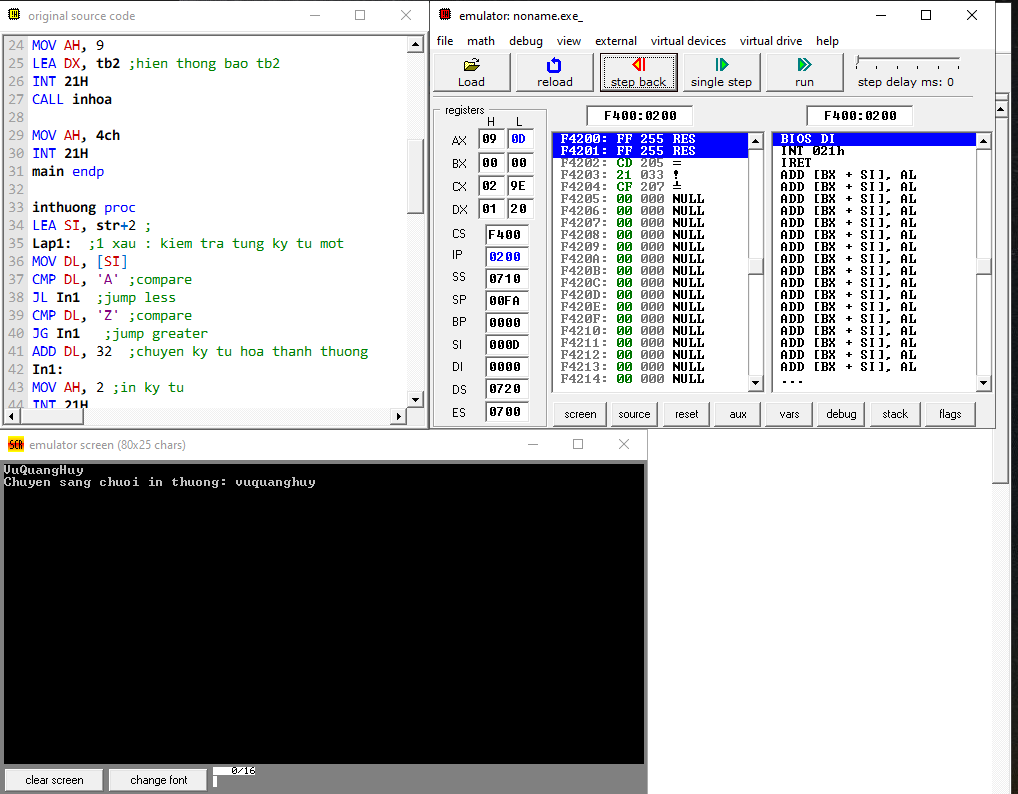
\includegraphics[width=0.9\textwidth]{Huy/2.2.4.png}
\end{figure}

\begin{figure}[H]
    \centering
    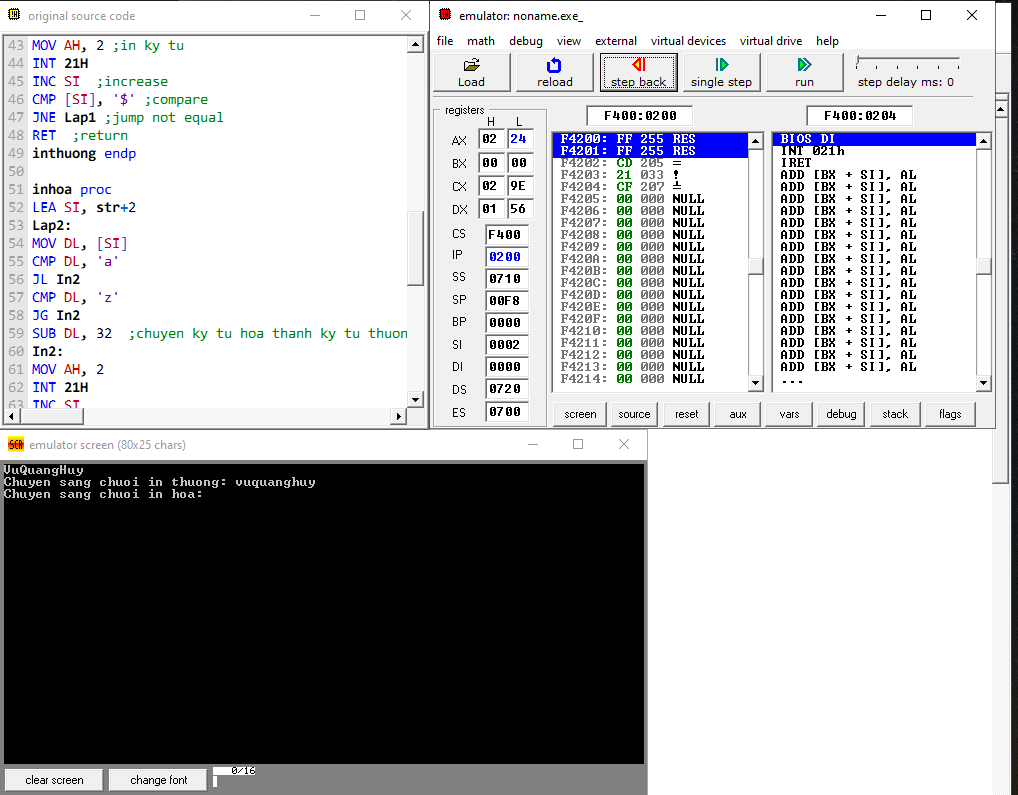
\includegraphics[width=0.9\textwidth]{Huy/2.2.5.png}
\end{figure}

\begin{figure}[H]
    \centering
    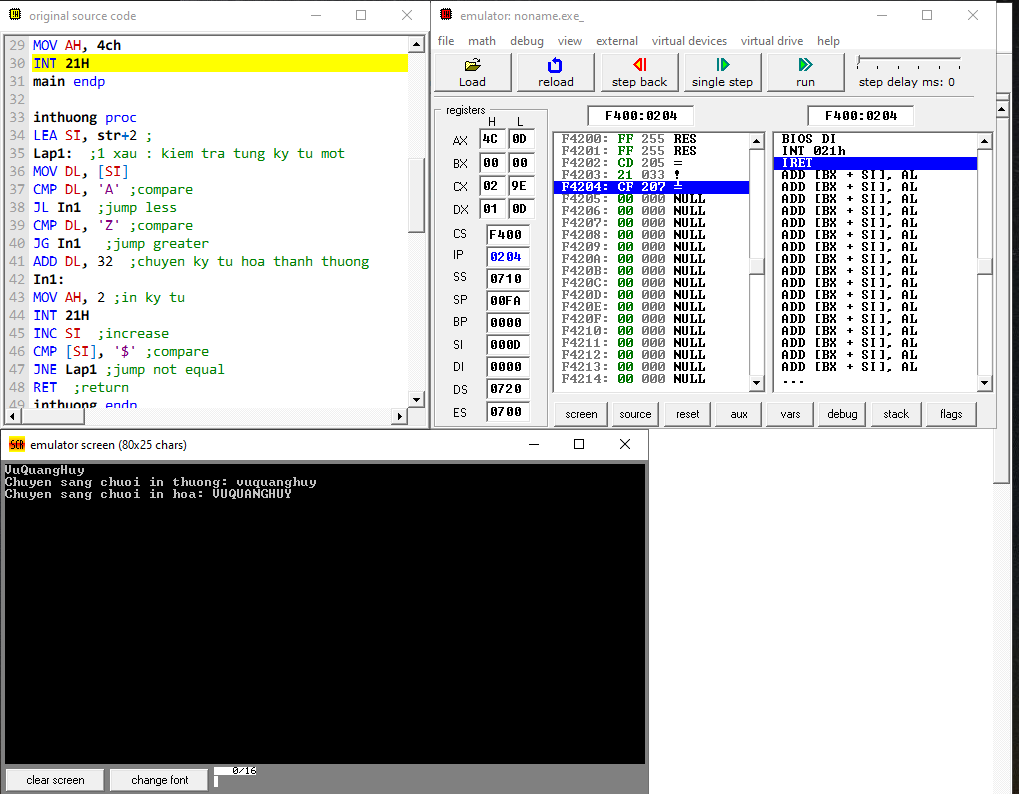
\includegraphics[width=0.9\textwidth]{Huy/2.2.6.png}
\end{figure}

\subsection{Giải thích nội dung các thanh ghi}
Khi chương trình bắt đầu chạy, hệ điều hành tự động khởi tạo các thanh ghi, vùng nhớ và cấp phát không gian địa chỉ cho chương trình. Tương ứng với các câu lệnh trong mã nguồn, nội dung các thanh ghi có thể thay đổi hoặc không.

\subsubsection{IP (Instruction Pointer)}
\begin{itemize}
    \item IP là thanh ghi trỏ đến địa chỉ của lệnh tiếp theo sẽ được thực thi trong mã máy.
    \item Khi một chương trình được thực thi, IP được cập nhật để trỏ đến lệnh tiếp theo trong mã nguồn. Điều này giúp CPU biết lệnh nào sẽ được thực thi tiếp theo.
\end{itemize}

\subsubsection{DS (Data Segment) và SI (Source Index)}
\begin{itemize}
    \item DS là thanh ghi chỉ đến phân đoạn dữ liệu, nơi dữ liệu chương trình được lưu trữ.
    \item SI thường được sử dụng trong các phép toán dữ liệu và là một trong các thanh ghi chỉ địa chỉ.
    \item Khi chương trình yêu cầu truy cập dữ liệu từ bộ nhớ, DS và SI thường được sử dụng để xác định vị trí của dữ liệu trong bộ nhớ.
\end{itemize}

\subsubsection{SS (Stack Segment) và BP (Base Pointer)}
\begin{itemize}
    \item SS là thanh ghi chỉ đến phân đoạn ngăn xếp (stack segment), nơi các giá trị cục bộ và địa chỉ của các hàm được lưu trữ.
    \item BP thường được sử dụng để trỏ đến địa chỉ cơ sở của ngăn xếp (base of stack).
    \item Ngăn xếp được sử dụng để lưu trữ các giá trị trung gian và địa chỉ trả về từ các hàm con (subroutines) trong quá trình thực thi chương trình.
\end{itemize}

\subsubsection{SP (Stack Pointer)}
\begin{itemize}
    \item SP là thanh ghi chỉ đến đỉnh của ngăn xếp (top of stack).
    \item Khi dữ liệu được đẩy (push) hoặc rút (pop) ra khỏi ngăn xếp, SP sẽ thay đổi để chỉ đến vị trí mới nhất trong ngăn xếp.
    \item SP cũng được sử dụng để cấp phát không gian mới cho dữ liệu trong ngăn xếp.
\end{itemize}

\subsection{Cơ chế quản lý bộ nhớ}

Cụ thể, trong trường hợp của đoạn chương trình chuyển xâu ký tự thành xâu in hoa và in thường tương ứng, ta có cơ chế quản lý bộ nhớ như sau:

\subsubsection{Khởi tạo bộ nhớ}
\begin{itemize}
    \item Khi chương trình bắt đầu, HĐH sẽ cấp phát các đoạn mã (code), dữ liệu (data), và ngăn xếp (stack) cho chương trình.
    \item Đoạn mã chứa các lệnh chương trình, đoạn dữ liệu chứa các biến, và đoạn ngăn xếp dùng để lưu trữ dữ liệu tạm thời.
\end{itemize}

\subsubsection{Phân đoạn bộ nhớ}
\begin{itemize}
    \item CS (Code Segment) trỏ tới đoạn mã của chương trình.
    \item DS (Data Segment) trỏ tới đoạn dữ liệu của chương trình.
    \item SS (Stack Segment) trỏ tới đoạn ngăn xếp của chương trình.
\end{itemize}

\subsubsection{Quản lý ngăn xếp}
\begin{itemize}
    \item Ngăn xếp được sử dụng để lưu trữ tạm thời dữ liệu và địa chỉ trả về khi gọi hàm.
    \item SP được khởi tạo với giá trị từ khai báo .Stack 100H, nghĩa là kích thước ngăn xếp là 256 byte.
\end{itemize}


\section{Lê Huy Hải}

\subsection{Khảo sát cấu hình máy}
Khảo sát cấu hình của máy và hệ thống bộ nhớ của máy đang sử dụng (Bộ nhớ trong: ROM, RAM, Cache System,..) được thực hiện bằng phần mềm CPU-Z.

\subsubsection{CPU}
\begin{figure}[H]
    \centering
    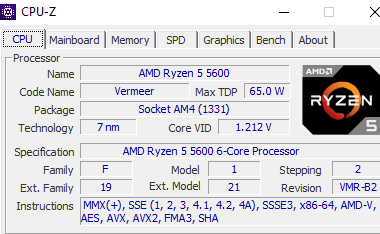
\includegraphics[width=0.8\textwidth]{Hải/Image_10.png}
    \caption{ADM-Ryzen 5-5600 – 6 nhân – 12 luồng.}
\end{figure}

\subsubsection{Cache}
\begin{figure}[H]
    \centering
    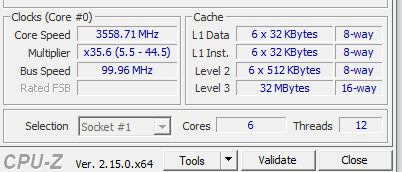
\includegraphics[width=0.9\textwidth]{Hải/Image_11.png}
    \caption{Hệ thống cache của máy tính bao gồm các cấp L1, L2, và L3.}
\end{figure}

\subsubsection{RAM}
\begin{figure}[H]
    \centering
    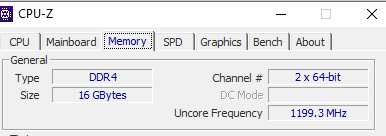
\includegraphics[width=0.9\textwidth]{Hải/Image_12.png}
    \caption{16Gb.}
\end{figure}

\subsubsection{Bộ nhớ ngoài}
\begin{figure}[H]
    \centering
    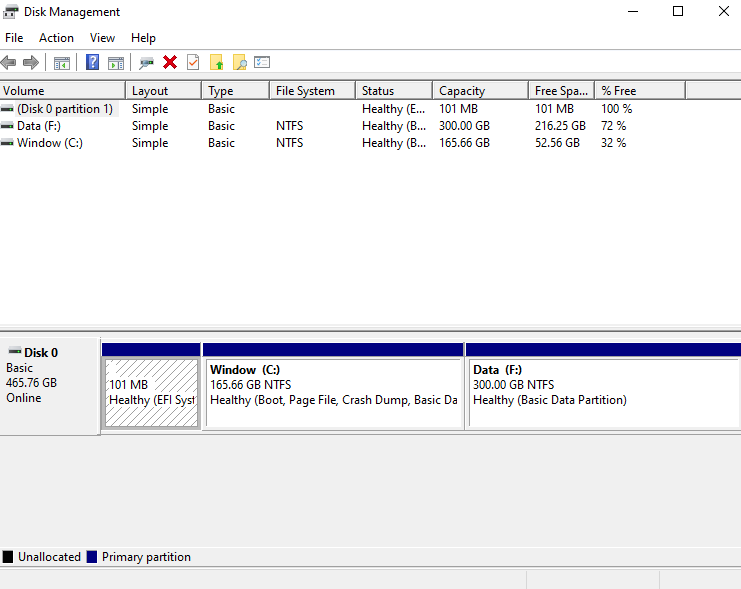
\includegraphics[width=0.9\textwidth]{Hải/Image_13.png}
\end{figure}

\subsubsection{Các thiết bị vào ra}
\begin{figure}[H]
    \centering
    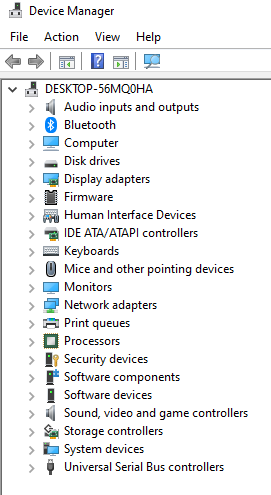
\includegraphics[width=0.7\textwidth]{Hải/Image_14.png}
    \caption{Các thiết bị vào ra bao gồm bàn phím, chuột, màn hình, và các cổng kết nối.}
\end{figure}


\subsection{Khảo sát nội dung các thanh ghi}


\subsubsection{Giải thích nội dung các thanh ghi}
Dùng công cụ Debug khảo sát nội dung các thanh ghi IP, DS, ES, SS, CS, BP, SP

\begin{itemize}
    \item Công cụ sử dụng: emu8086 microprocessor emulator
    \item Các bước thực hiện:
    \item Mở file .asm bằng phần mềm trên
    \item Chọn emulate trên thanh công cụ rồi chọn nút debug nằm cuối của cửa sổ vừa mở ra
    \item Chạy Single step để xem kết quả debug từng mã lệnh từ đầu đến cuối
\end{itemize}

\begin{figure}[H]
    \centering
    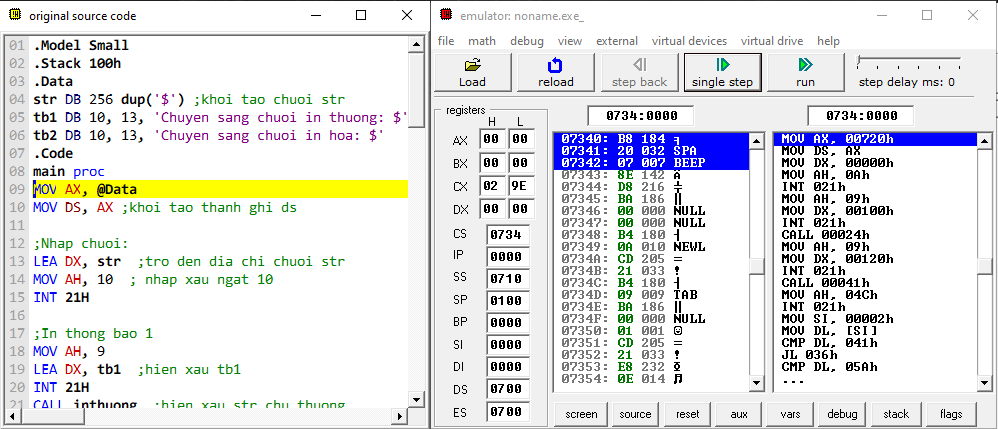
\includegraphics[width=1\textwidth]{Hải/Image_15.png}
\end{figure}

\begin{figure}[H]
    \centering
    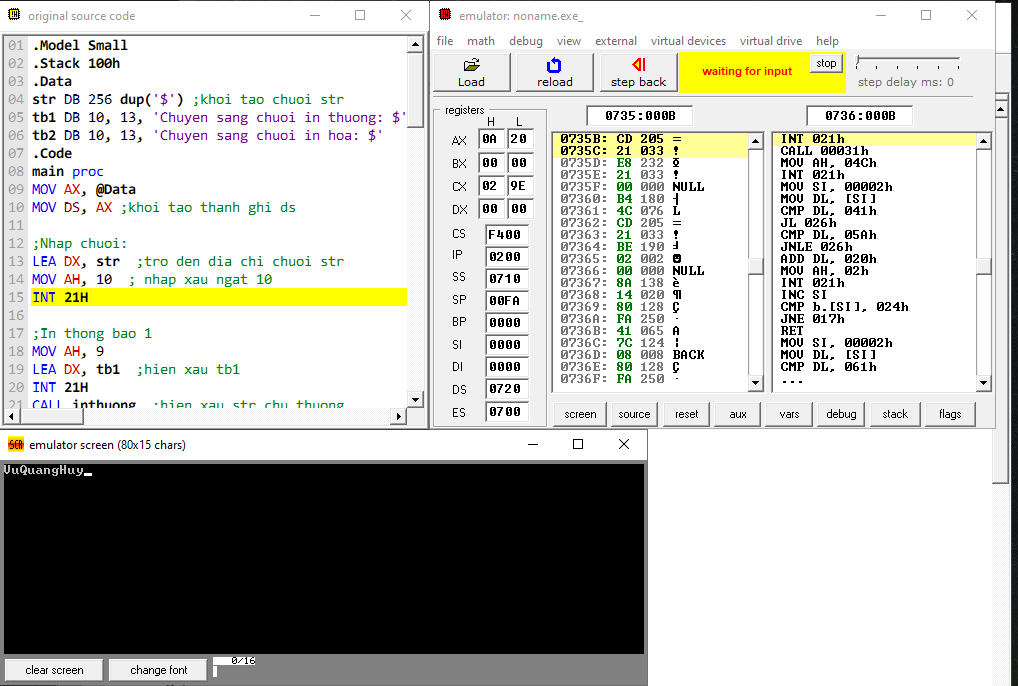
\includegraphics[width=0.95\textwidth]{Hải/Image_16.png}
\end{figure}

\begin{figure}[H]
    \centering
    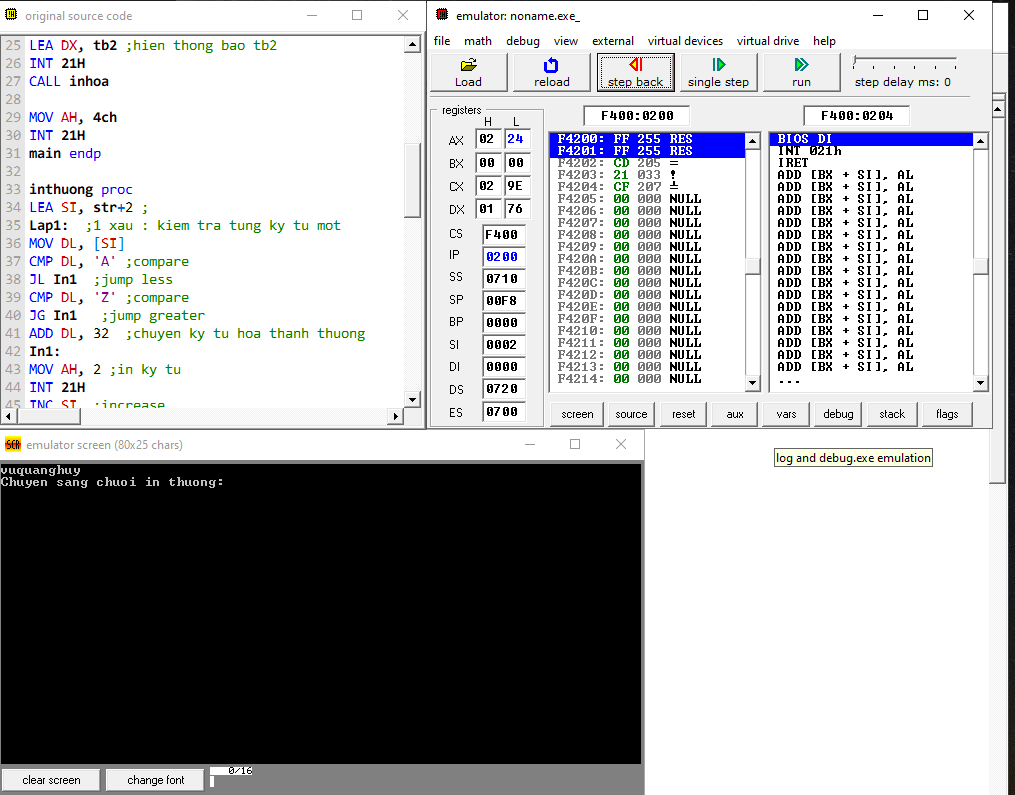
\includegraphics[width=0.95\textwidth]{Hải/Image_17.png}
\end{figure}

\begin{figure}[H]
    \centering
    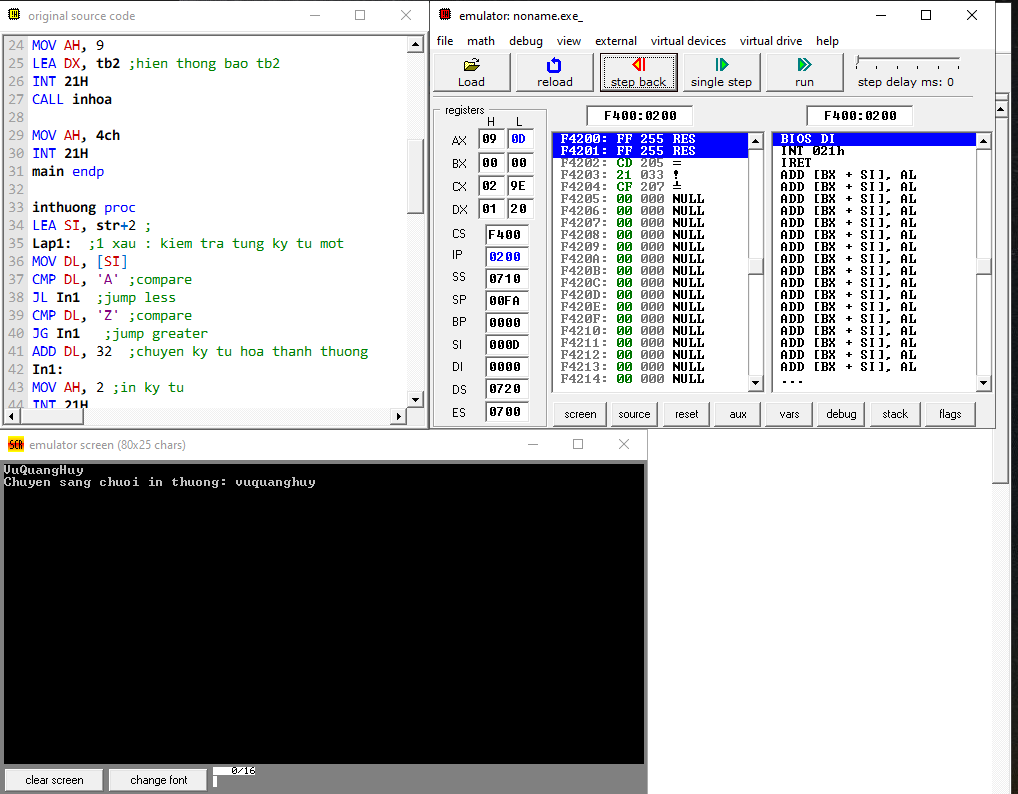
\includegraphics[width=0.9\textwidth]{Hải/Image_18.png}
\end{figure}

\begin{figure}[H]
    \centering
    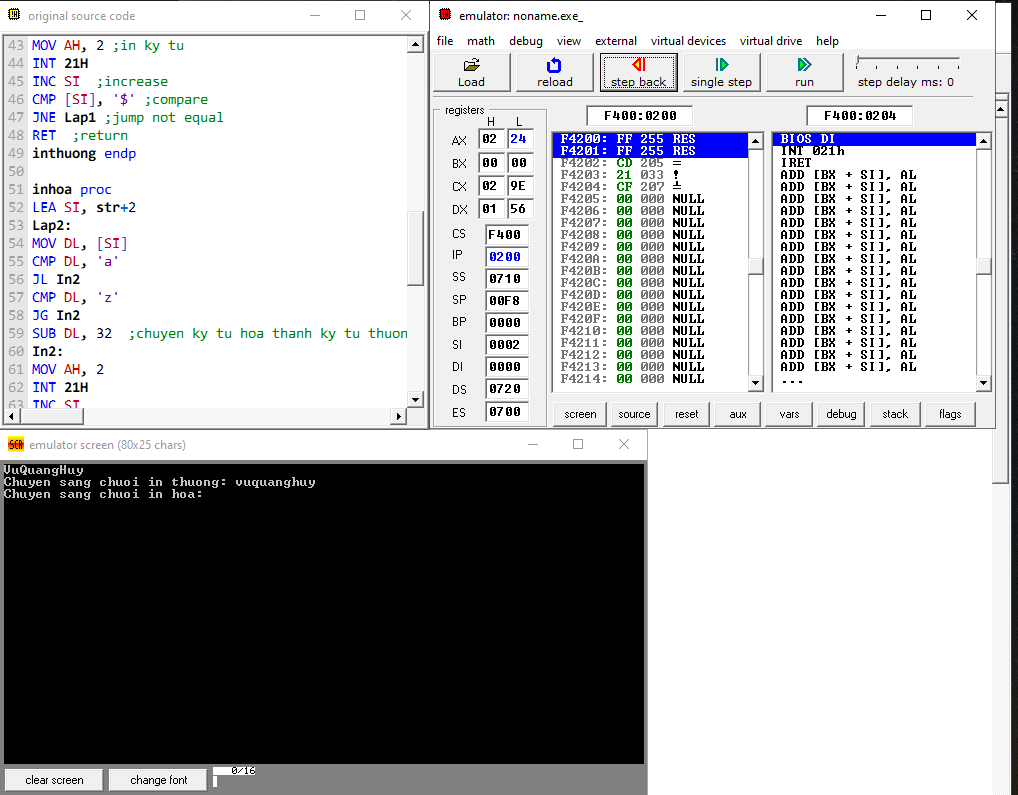
\includegraphics[width=0.9\textwidth]{Hải/Image_19.png}
\end{figure}

\begin{figure}[H]
    \centering
    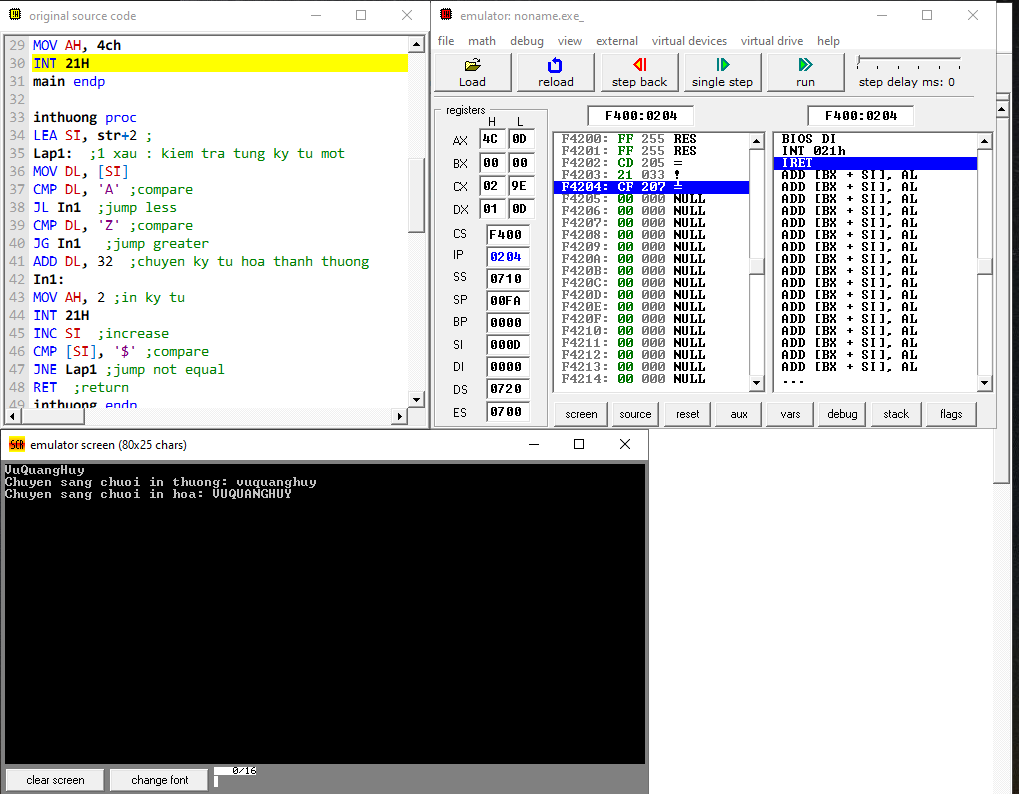
\includegraphics[width=1\textwidth]{Hải/Image_20.png}
\end{figure}


\subsection{Giải thích nội dung các thanh ghi}
Khi chương trình bắt đầu chạy, hệ điều hành tự động khởi tạo các thanh ghi, vùng nhớ và cấp phát không gian địa chỉ cho chương trình. Tương ứng với các câu lệnh trong mã nguồn, nội dung các thanh ghi có thể thay đổi hoặc không.

\subsubsection{IP (Instruction Pointer)}
\begin{itemize}
    \item IP là thanh ghi trỏ đến địa chỉ của lệnh tiếp theo sẽ được thực thi trong mã máy.
    \item Khi một chương trình được thực thi, IP được cập nhật để trỏ đến lệnh tiếp theo trong mã nguồn. Điều này giúp CPU biết lệnh nào sẽ được thực thi tiếp theo.
\end{itemize}

\subsubsection{DS (Data Segment) và SI (Source Index)}
\begin{itemize}
    \item DS là thanh ghi chỉ đến phân đoạn dữ liệu, nơi dữ liệu chương trình được lưu trữ.
    \item SI thường được sử dụng trong các phép toán dữ liệu và là một trong các thanh ghi chỉ địa chỉ.
    \item Khi chương trình yêu cầu truy cập dữ liệu từ bộ nhớ, DS và SI thường được sử dụng để xác định vị trí của dữ liệu trong bộ nhớ.
\end{itemize}

\subsubsection{SS (Stack Segment) và BP (Base Pointer)}
\begin{itemize}
    \item SS là thanh ghi chỉ đến phân đoạn ngăn xếp (stack segment), nơi các giá trị cục bộ và địa chỉ của các hàm được lưu trữ.
    \item BP thường được sử dụng để trỏ đến địa chỉ cơ sở của ngăn xếp (base of stack).
    \item Ngăn xếp được sử dụng để lưu trữ các giá trị trung gian và địa chỉ trả về từ các hàm con (subroutines) trong quá trình thực thi chương trình.
\end{itemize}

\subsubsection{SP (Stack Pointer)}
\begin{itemize}
    \item SP là thanh ghi chỉ đến đỉnh của ngăn xếp (top of stack).
    \item Khi dữ liệu được đẩy (push) hoặc rút (pop) ra khỏi ngăn xếp, SP sẽ thay đổi để chỉ đến vị trí mới nhất trong ngăn xếp.
    \item SP cũng được sử dụng để cấp phát không gian mới cho dữ liệu trong ngăn xếp.
\end{itemize}

\subsection{Cơ chế quản lý bộ nhớ}

Cụ thể, trong trường hợp của đoạn chương trình chuyển xâu ký tự thành xâu in hoa và in thường tương ứng, ta có cơ chế quản lý bộ nhớ như sau:

\subsubsection{Khởi tạo bộ nhớ}
\begin{itemize}
    \item Khi chương trình bắt đầu, HĐH sẽ cấp phát các đoạn mã (code), dữ liệu (data), và ngăn xếp (stack) cho chương trình.
    \item Đoạn mã chứa các lệnh chương trình, đoạn dữ liệu chứa các biến, và đoạn ngăn xếp dùng để lưu trữ dữ liệu tạm thời.
\end{itemize}

\subsubsection{Phân đoạn bộ nhớ}
\begin{itemize}
    \item CS (Code Segment) trỏ tới đoạn mã của chương trình.
    \item DS (Data Segment) trỏ tới đoạn dữ liệu của chương trình.
    \item SS (Stack Segment) trỏ tới đoạn ngăn xếp của chương trình.
\end{itemize}

\subsubsection{Quản lý ngăn xếp}
\begin{itemize}
    \item Ngăn xếp được sử dụng để lưu trữ tạm thời dữ liệu và địa chỉ trả về khi gọi hàm.
    \item SP được khởi tạo với giá trị từ khai báo .Stack 100H, nghĩa là kích thước ngăn xếp là 256 byte.
\end{itemize}




\section{Hà Duy Khánh}

\subsection{Khảo sát cấu hình máy}
Khảo sát cấu hình của máy và hệ thống bộ nhớ của máy đang sử dụng (Bộ nhớ trong: ROM, RAM, Cache System,..) được thực hiện bằng phần mềm CPU-Z.



\subsubsection{CPU}
\begin{figure}[H]
    \centering
    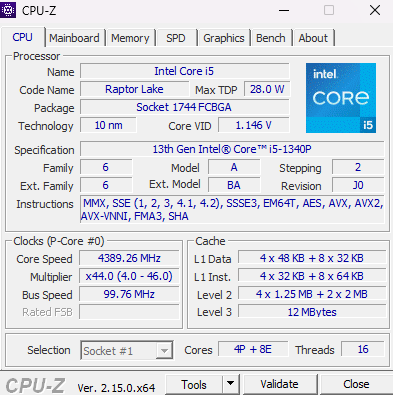
\includegraphics[width=0.8\textwidth]{Khánh/8.png}
    \caption{Intel Core i5 - 12 nhân - 16 luồng.}
\end{figure}

\subsubsection{Cache}
\begin{figure}[H]
    \centering
    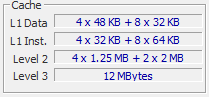
\includegraphics[width=0.8\textwidth]{Khánh/9.png}
    \caption{Hệ thống cache của máy tính bao gồm các cấp L1, L2, và L3}
\end{figure}

\subsubsection{RAM}
\begin{figure}[H]
    \centering
    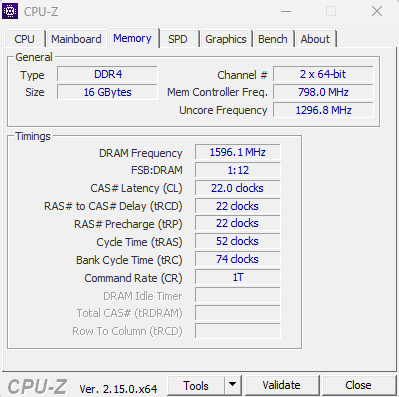
\includegraphics[width=0.7\textwidth]{Khánh/10.png}
    \caption{16Gb.}
\end{figure}


\subsubsection{Bộ nhớ ngoài}
\begin{figure}[H]
    \centering
    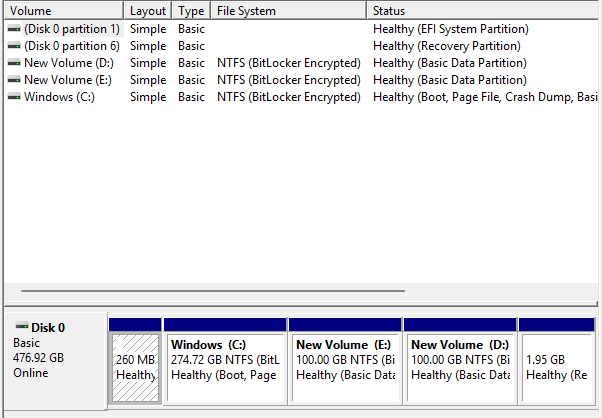
\includegraphics[width=0.8\textwidth]{Khánh/11.png}
\end{figure}


\subsubsection{Các thiết bị vào ra}
\begin{figure}[H]
    \centering
    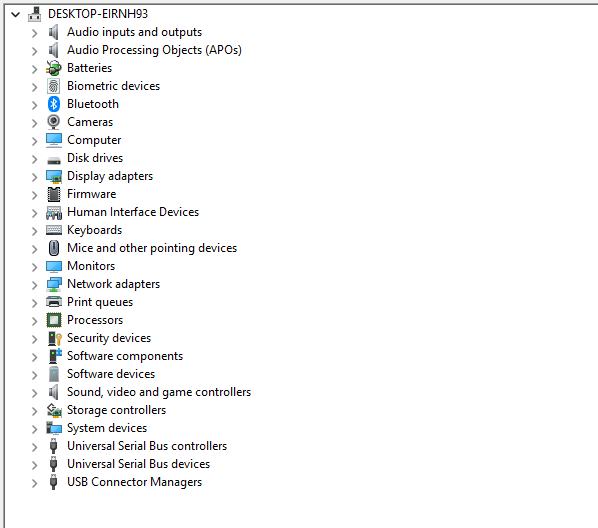
\includegraphics[width=0.8\textwidth]{Khánh/12.png}
    \caption{Bao gồm bàn phím, chuột, màn hình, và các cổng kết nối.}
\end{figure}


\subsection{Khảo sát nội dung các thanh ghi}


\subsubsection{Giải thích nội dung các thanh ghi}
Dùng công cụ Debug khảo sát nội dung các thanh ghi IP, DS, ES, SS, CS, BP, SP

\begin{itemize}
    \item Công cụ sử dụng: emu8086 microprocessor emulator
    \item Các bước thực hiện:
    \item Mở file .asm bằng phần mềm trên
    \item Chọn emulate trên thanh công cụ rồi chọn nút debug nằm cuối của cửa sổ vừa mở ra
    \item Chạy Single step để xem kết quả debug từng mã lệnh từ đầu đến cuối
\end{itemize}

\begin{figure}[H]
    \centering
    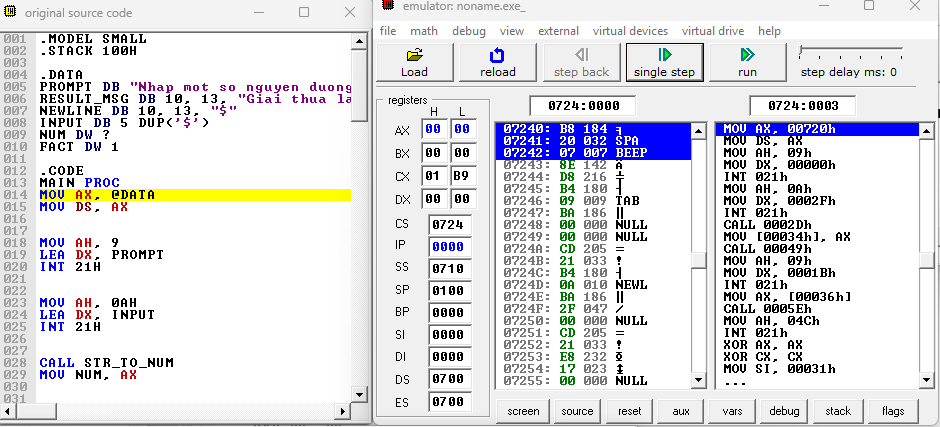
\includegraphics[width=1\textwidth]{Khánh/13.png}
\end{figure}

\begin{figure}[H]
    \centering
    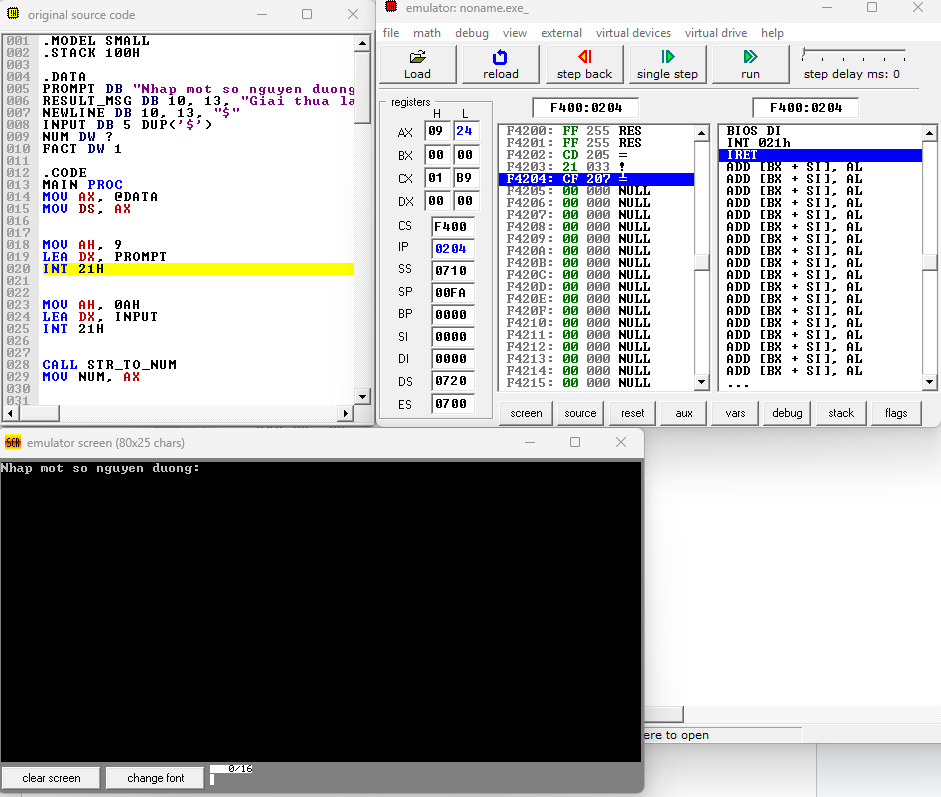
\includegraphics[width=1\textwidth]{Khánh/14.png}
\end{figure}

\begin{figure}[H]
    \centering
    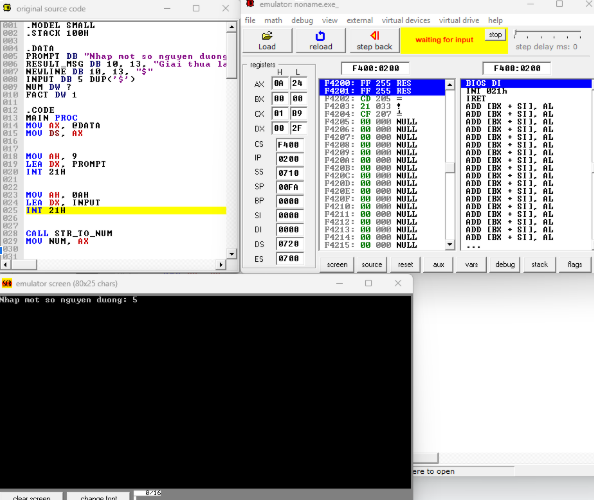
\includegraphics[width=0.85\textwidth]{Khánh/15.png}
\end{figure}

\begin{figure}[H]
    \centering
    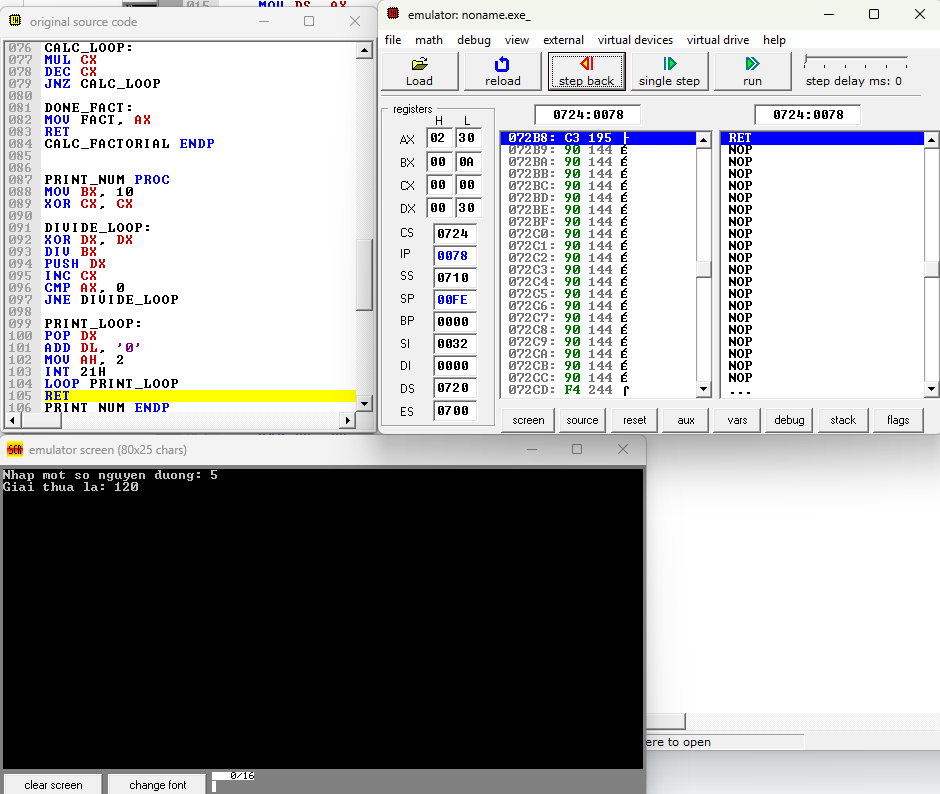
\includegraphics[width=0.85\textwidth]{Khánh/16.png}
\end{figure}


\subsection{Giải thích nội dung các thanh ghi}
Khi chương trình bắt đầu chạy, hệ điều hành tự động khởi tạo các thanh ghi, vùng nhớ và cấp phát không gian địa chỉ cho chương trình. Tương ứng với các câu lệnh trong mã nguồn, nội dung các thanh ghi có thể thay đổi hoặc không.

\subsubsection{IP (Instruction Pointer)}
\begin{itemize}
    \item IP là thanh ghi trỏ đến địa chỉ của lệnh tiếp theo sẽ được thực thi trong mã máy.
    \item Khi một chương trình được thực thi, IP được cập nhật để trỏ đến lệnh tiếp theo trong mã nguồn. Điều này giúp CPU biết lệnh nào sẽ được thực thi tiếp theo.
\end{itemize}

\subsubsection{DS (Data Segment) và SI (Source Index)}
\begin{itemize}
    \item DS là thanh ghi chỉ đến phân đoạn dữ liệu, nơi dữ liệu chương trình được lưu trữ.
    \item SI thường được sử dụng trong các phép toán dữ liệu và là một trong các thanh ghi chỉ địa chỉ.
    \item Khi chương trình yêu cầu truy cập dữ liệu từ bộ nhớ, DS và SI thường được sử dụng để xác định vị trí của dữ liệu trong bộ nhớ.
\end{itemize}

\subsubsection{SS (Stack Segment) và BP (Base Pointer)}
\begin{itemize}
    \item SS là thanh ghi chỉ đến phân đoạn ngăn xếp (stack segment), nơi các giá trị cục bộ và địa chỉ của các hàm được lưu trữ.
    \item BP thường được sử dụng để trỏ đến địa chỉ cơ sở của ngăn xếp (base of stack).
    \item Ngăn xếp được sử dụng để lưu trữ các giá trị trung gian và địa chỉ trả về từ các hàm con (subroutines) trong quá trình thực thi chương trình.
\end{itemize}

\subsubsection{SP (Stack Pointer)}
\begin{itemize}
    \item SP là thanh ghi chỉ đến đỉnh của ngăn xếp (top of stack).
    \item Khi dữ liệu được đẩy (push) hoặc rút (pop) ra khỏi ngăn xếp, SP sẽ thay đổi để chỉ đến vị trí mới nhất trong ngăn xếp.
    \item SP cũng được sử dụng để cấp phát không gian mới cho dữ liệu trong ngăn xếp.
\end{itemize}

\subsection{Cơ chế quản lý bộ nhớ}

Cụ thể, trong trường hợp của đoạn chương trình chuyển xâu ký tự thành xâu in hoa và in thường tương ứng, ta có cơ chế quản lý bộ nhớ như sau:

\subsubsection{Khởi tạo bộ nhớ}
\begin{itemize}
    \item Khi chương trình bắt đầu, HĐH sẽ cấp phát các đoạn mã (code), dữ liệu (data), và ngăn xếp (stack) cho chương trình.
    \item Đoạn mã chứa các lệnh chương trình, đoạn dữ liệu chứa các biến, và đoạn ngăn xếp dùng để lưu trữ dữ liệu tạm thời.
\end{itemize}

\subsubsection{Phân đoạn bộ nhớ}
\begin{itemize}
    \item CS (Code Segment) trỏ tới đoạn mã của chương trình.
    \item DS (Data Segment) trỏ tới đoạn dữ liệu của chương trình.
    \item SS (Stack Segment) trỏ tới đoạn ngăn xếp của chương trình.
\end{itemize}

\subsubsection{Quản lý ngăn xếp}
\begin{itemize}
    \item Ngăn xếp được sử dụng để lưu trữ tạm thời dữ liệu và địa chỉ trả về khi gọi hàm.
    \item SP được khởi tạo với giá trị từ khai báo .Stack 100H, nghĩa là kích thước ngăn xếp là 256 byte.
\end{itemize}





\chapter*{Kết luận}
\addcontentsline{toc}{chapter}{Kết luận} 
\markboth{Kết luận}{}

Qua quá trình thực hiện các bài tập lập trình hợp ngữ Assembly và phân tích khảo sát hệ thống bộ nhớ, chúng tôi đã đạt được những kết quả và kiến thức quan trọng sau:

Về lập trình hợp ngữ Assembly, chúng tôi đã thực hiện thành công nhiều bài tập đa dạng như chuyển đổi ký tự thường thành hoa, chuyển đổi giữa các hệ cơ số, tính toán số học, và xử lý chuỗi. Qua đó, chúng tôi đã hiểu sâu hơn về cách thức hoạt động của các lệnh Assembly, cách tổ chức và quản lý dữ liệu, cũng như các kỹ thuật lập trình cấp thấp.

Về phân tích khảo sát hệ thống bộ nhớ, chúng tôi đã tìm hiểu và phân tích cấu hình máy tính, bao gồm CPU, cache, RAM, và các thiết bị lưu trữ. Đồng thời, chúng tôi cũng đã khảo sát và giải thích nội dung các thanh ghi như IP, DS, ES, SS, CS, BP, SP, từ đó hiểu rõ hơn về cơ chế quản lý bộ nhớ của hệ thống. Việc này giúp chúng tôi nắm vững kiến thức về kiến trúc máy tính và cách thức hoạt động của bộ nhớ.

Những kiến thức và kỹ năng thu được từ đồ án này không chỉ giúp chúng tôi hiểu sâu hơn về lập trình cấp thấp và kiến trúc máy tính, mà còn là nền tảng quan trọng cho việc học tập và nghiên cứu các môn học khác trong lĩnh vực khoa học máy tính. Đặc biệt, việc hiểu rõ về cách thức hoạt động của máy tính ở mức thấp sẽ giúp chúng tôi phát triển phần mềm hiệu quả và tối ưu hơn trong tương lai.

Tuy nhiên, chúng tôi cũng nhận thấy rằng còn nhiều vấn đề phức tạp và sâu sắc hơn trong lĩnh vực lập trình Assembly và kiến trúc máy tính cần được tiếp tục nghiên cứu và tìm hiểu. Trong tương lai, chúng tôi hy vọng sẽ có cơ hội để mở rộng kiến thức và kỹ năng trong lĩnh vực này, đặc biệt là trong các ứng dụng thực tế như tối ưu hóa hiệu suất, phát triển hệ thống nhúng, và bảo mật hệ thống.

\end{document}
